\documentclass[10pt,twocolumn,letterpaper]{article}

\usepackage{cvpr}
\usepackage{times}
\usepackage{epsfig}
\usepackage{graphicx}
\usepackage{amsmath}
\usepackage{amssymb}
\usepackage{array}
\usepackage{caption}
\usepackage{subcaption}
\usepackage{tikz}
\usepackage{pgfplots}
\pgfplotsset{compat=1.7}


% Include other packages here, before hyperref.

% If you comment hyperref and then uncomment it, you should delete
% egpaper.aux before re-running latex.  (Or just hit 'q' on the first latex
% run, let it finish, and you should be clear).
\usepackage[breaklinks=true]{hyperref}
\hypersetup{
  % bookmarks=false,
  bookmarksnumbered=true,
  pdfauthor={Andrea Esposito, Graziano Montanaro},
  pdftitle={Diagnosing Dementia Through the Automatic Analysis of Amyloid PET Scans},
}
\usepackage[noabbrev]{cleveref}

\cvprfinalcopy % *** Uncomment this line for the final submission

\def\cvprPaperID{****} % *** Enter the CVPR Paper ID here
\def\httilde{\mbox{\tt\raisebox{-.5ex}{\symbol{126}}}}

% Pages are numbered in submission mode, and unnumbered in camera-ready
\ifcvprfinal\pagestyle{empty}\fi
%\setcounter{page}{4321}
\begin{document}

%%%%%%%%% TITLE
\title{Diagnosing Dementia Through the Automatic Analysis of Amyloid PET Scans}

\author{%
  Andrea Esposito\\
  University of Bari ``A. Moro''\\
  Department of Computer Science\\
  {\tt\small a.esposito39@studenti.uniba.it}
  \and
  Graziano Montanaro\\
  University of Bari ``A. Moro''\\
  Department of Computer Science\\
  {\tt\small g.montanaro16@studenti.uniba.it}
}

\maketitle
%\thispagestyle{empty}

%%%%%%%%% ABSTRACT
\begin{abstract}
  Dementia is one of the most common diseases in the elderly and one of the
  major causes of mortality and disability: from European studies conducted in
  2000, the estimated prevalence of dementia in the elderly (over 65 years old)
  was 6.4\%, among which the most prevalent cause is Alzheimer's Disease
  followed by vascular dementia. This paper aims at proposing a modular model
  that allows the diagnosis of dementia, although the proposed approach is still
  in an embryonic stage, by analyzing images obtained through Magnetic Resonance
  Imaging (MRI) through Computer Vision techniques using Artificial Neural
  Networks. To fit in the strict schedule of this paper, the proposed model will
  not be implemented in its entirety: since Alzheimer's disease is the prevalent
  cause of dementia, the implemented model is only able to diagnose dementia due
  to the aforementioned disease.
\end{abstract}

\section{Introduction}
\label{sec:introduction}


Dementia is one of the most common diseases in the elderly and one of the major
causes of mortality and disability \cite{Berr2005}: from European studies
conducted in 2000, the estimated prevalence of dementia in the elderly (over 65
years old) was 6.4\% \cite{Barkhof2016}, among which the most prevalent cause is
Alzheimer's Disease followed by vascular dementia \cite{Barkhof2016}.

To diagnose dementia, a better overview of what it is must be given. Dementia is
not a syndrome, but rather a symptom of an underlying pathology that depends on
the age of the patient \cite{Barkhof2016}. For example, in younger patients,
Huntington's disease and genetic forms of Alzheimer's disease tend to occur more
often, while in older patients cognitive problems are often due to Alzheimer's
disease, Lewy body dementia, and vascular diseases
\cite{Barkhof2016,Knopman2006}.

This paper aims at contributing to a modular model that allows the diagnosis of
dementia, although the proposed approach is still in an embryonic stage, using 
Magnetic Resonance scans, PET scans and personal data (like age and sex). To
reach the proposed goal, we chose to analyze images obtained through PET
(Positron-Emittion Tomography) scans through Computer Vision techniques using
Artificial Neural Networks. In fact, various diseases that cause dementia often
share findings and anomalies in PET and Magnetic Resonance images: anomalies in
glucose metabolism, presence of amyloid placques, and atrophies in different
parts of the brain are, for example, clues of Alzheimer's disease,
frontotemporal lobe degeneration, and corticobasal degeneration, while lesions
in the white or gray matter of the brain are indicators of infections or
metabolic diseases \cite{Barkhof2016,Chetelat2020}.

To fit in the strict schedule of this paper, the proposed model will not be
implemented in its entirety: since Alzheimer's disease is the prevalent cause of
dementia, the implemented model is only able to diagnose dementia due to the
aforementioned disease. Such implementation will be further discussed in
\cref{sec:methods} and evaluated in \cref{sec:experiments}.

The paper is organized as follows: \cref{sec:related-work} discusses the
rationale and background of the proposed approach; \cref{sec:data} presents and
discusses the dataset used to train and test the model built using the methods
discussed in \cref{sec:methods}. Finally, \cref{sec:experiments} details the
testing phase and its results, while \cref{sec:conclusions} provides the
conclusions and highlights the possible improvements for future works.

\section{Related Work}
\label{sec:related-work}

Dementia was the second greatest source of disability burden in Australia in
2008 \cite{Speechly2008}. An accurate and early diagnosis allows the
implementation of an intervention to slow the progression of the disease and
even cure it, when possible \cite{Speechly2008}. Sadly, the time between the
onset of symptoms and the diagnosis is often long \cite{Fiske2005}, due to the
insidious onset of the disease and the under-recognition or uncertainty by
families about the path to diagnosis \cite{Speechly2008}. Various attempts have
been made in the medical field to diagnose neurodegenerative diseases and, more
specifically, dementia as soon as possible, and Artificial Intelligence aims at
helping diagnosticians recognize the underlying diseases that wither the
patients' cognitive abilities.

\begin{figure}[htb]
  \resizebox{\linewidth}{!}{%
    \begin{tabular}{>{\centering\arraybackslash}m{1.7cm}>{\centering\arraybackslash}m{.2\linewidth}>{\centering\arraybackslash}m{.2\linewidth}>{\centering\arraybackslash}m{.2\linewidth}}
                                  & Atrophy                                                                    & Glucose Metabolism                                                             & Amyloid $\beta$ \\
      \textbf{Healthy}             & 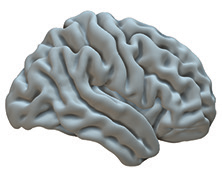
\includegraphics[width=\linewidth]{images/healthy-vs-ad/healthy/mri.png}   & 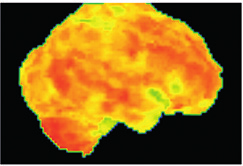
\includegraphics[width=\linewidth]{images/healthy-vs-ad/healthy/glucose.png}   & 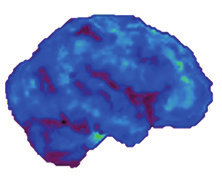
\includegraphics[width=\linewidth]{images/healthy-vs-ad/healthy/amyloid.png} \\
      \textbf{Alzheimer's Disease} & 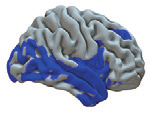
\includegraphics[width=\linewidth]{images/healthy-vs-ad/alzheimer/mri.png} & 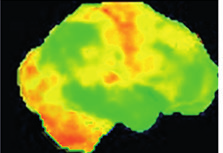
\includegraphics[width=\linewidth]{images/healthy-vs-ad/alzheimer/glucose.png} & 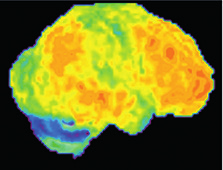
\includegraphics[width=\linewidth]{images/healthy-vs-ad/alzheimer/amyloid.png} \\
                                  & Structural MRI                                                             & FDG-PET                                                                        & Amyloid-PET \\
    \end{tabular}
  }
  \caption{Neuroimaging obtained with structural MRI or PET using different radiotracers in both healthy subject and subjects affected by Alzheimer's disease (adapted from \cite{Chetelat2020})}
  \label{fig:healthy-vs-ad}
\end{figure}

Among the attempts at diagnosing dementia in a pre-clinical stage, the work
presented in \cite{Altay2020} presents a diagnostic model based on the analysis
of MRI scans of the brain, starting from the OASIS3 dataset
\cite{LaMontagne2019}. Although the usage of MRI scans is effective in the
search of scar tissues, necrosis, and/or atrophies in the brain, recent
researches has shown an high correlation between the quantity of
amyloid\footnote{``Amyloid'' denotes peptides of 36 to 43 amino acids whose
  function is not yet fully understood \cite{Hiltunen2009}.} in the brain cortex
and Alzheimer's disease \cite{Chetelat2020}.

In the medical field, PET scans are classified using the contrast material. The
three PET scans heavily used in Alzheimer's diagnosis and recognition are
PiB-PETs, AV45-PET, and FDG-PET \cite{Rice2017}. The main difference between
each of the three types of PET scans lays in the substance used as contrast
material: the PiB-PET scans use the Pittsburgh compound B (PiB) that binds to
amyloid, which tends to be concentrated near the brains' cortex of people
affected with Alzheimer's disease \cite{Klunk2004}; the AV45-PET scans use
florbetapir (AV45) that, similarly to PIB, binds to amyloid \cite{Camus2012};
lastly, the FDG-PET scans use fluorodeoxyglucose that, differently from the
previous compounds, is used to evaluate the metabolism of glucose
\cite{Newberg2002}. Between the three, amyloid PETs are slightly more sentitive
when used to diagnose Alzheimer's disease, especially in patients with known
histopathology \cite{Rabinovici2011}.

Sadly, to the extent of our knowledge, very few (or none) attempts have been
made yet at creating an automatic diagnostic tool for dementia and, more
specifically, Alzheimer's disease using amyloid concentration. Even fewer works
are based on the analysis of PET images, both for the evaluation of glucose's
metabolism and for the quantity of amyloid.


\section{Data}
\label{sec:data}

We chose to use the OASIS3 dataset, the latest version of the OASIS dataset that
was used by various authors for brain segmentation tasks \cite{Dalca2019,
  Huo2018, Huo2019, Rebsamen2020}, as it is a compilation of MRI and PET imaging
for 1098 participants, which include 605 cognitively normal adults and 493
individuals at various stages of cognitive decline ranging in age from 42 to 95
years \cite{LaMontagne2019}. To provide the most accurate diagnosis, both the
MRI and the PET scans should be analyzed. But, only the PET scans will be
considered to fit the time requirements for this work.

The dataset is made of 2168 MRI sessions and 1607 PET sessions, that can be used
to diagnose Alzheimer's disease as shown in \cref{fig:healthy-vs-ad}. We'll be
taking into consideration the 1352 PET sessions that have been already
post-processed, using the PET Unified Pipeline (PUP), available as part of the
dataset \cite{LaMontagne2019}. The OASIS3 dataset provides three different types
of PET scans, with different availability for every session: PiB-PETs, AV45-PET,
and FDG-PET \cite{LaMontagne2019}. For the scope of the work presented in this
paper, we'll only use the amyloid PET scans (i.e., the PiB-PET scans and the
AV45-PET scans), which comprise around 93\% of the entire PET scans dataset, as
FDG PETs have already been used in a similar context \cite{Singh2017}.

From an initial analysis of the available processed PET scans, for each scan
session, multiple images are provided (like the PET itself and an associated
T1-weighted MRI). From the perspective of this paper, only the PET scans
themselves are considered: more precisely, only the normalized motion-corrected
scans will be used.

\subsection{Labeling the Ground Truth}
\label{sec:labeling-ground-truth}

The OASIS3 dataset does not provide pre-labeled images, thus a labeling phase
was needed to provide the ground truth of the diagnostic model. The OASIS3
dataset provides for each patient a list of psychiatric and neurological
assessments alongside an evaluation of the cognitive state, using the Clinical
Dementia Rating (CDR) scale \cite{Morris1997}, and a possible diagnosis.

First, a pre-processing step of the dataset of diagnosis has to be executed:
each entry is labeled with up to five different differential diagnoses expressed
in natural language. First, all the labels have been mapped to either a value of
0 (that represents the ``healthy'' or ``non-dementia diagnosis'' cases) or a
value of 1 (that represents the ``Alzheimer's Disease or similar dementia
diagnosis'' cases), thus transforming the problem into a binary classification.
Then, after this first step, all the five differential diagnoses have been
merged into a single label, such that the final value is 1 if and only if at
least one differential diagnosis is in the ``Alzheimer's Disease or similar
dementia diagnosis'' class. To further improve this step, each label has then
been post-processed to remove the most false-negatives and false-positives from
the dataset: if the label is negative and at least one of the two predecessors
is positive and at least one of the two successors is positive, then the label
is switched to positive; otherwise, if the label is positive and the immediate
predecessor is not positive and the two successors are both negative, then the
label is switched to negative. The plot in
\autoref{fig:post-processing-for-false-classification} represents the results of
this post-processing phase.

\begin{figure}[h]
  \centering
  \begin{subfigure}[t]{\linewidth}
    \centering
    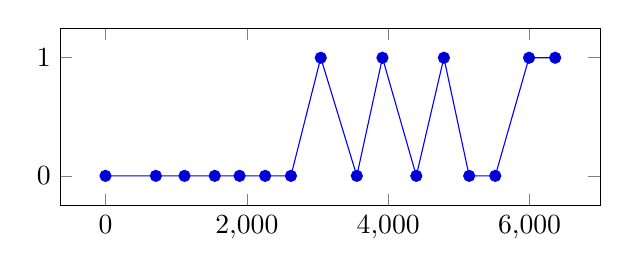
\begin{tikzpicture}
      \begin{axis}[
        ytick = {0, 1},
        y = 1.5cm,
        ymax = 1.25,
        ymin = -0.25
        ]
        \addplot coordinates {
          (0, 0) (713, 0) (1118, 0) (1546, 0) (1897, 0) (2259, 0) (2624, 0) (3046, 1) (3556, 0) (3919, 1) (4398, 0) (4788, 1) (5146, 0) (5515, 0) (5993, 1) (6363, 1)
        };
      \end{axis}
    \end{tikzpicture}
    \caption{Before}
  \end{subfigure}
  \begin{subfigure}[t]{\linewidth}
    \centering
    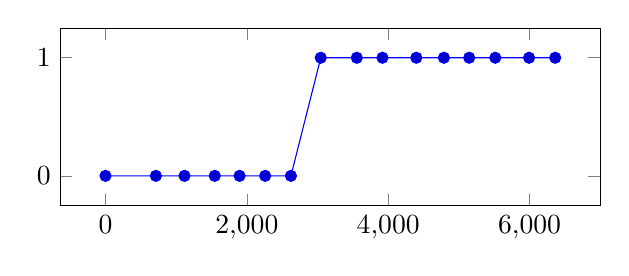
\begin{tikzpicture}
      \begin{axis}[
        ytick = {0, 1},
        y = 1.5cm,
        ymax = 1.25,
        ymin = -0.25
        ]
        \addplot coordinates {
          (0, 0) (713, 0) (1118, 0) (1546, 0) (1897, 0) (2259, 0) (2624, 0) (3046, 1) (3556, 1) (3919, 1) (4398, 1) (4788, 1) (5146, 1) (5515, 1) (5993, 1) (6363, 1)
        };
      \end{axis}
    \end{tikzpicture}
    \caption{After}
  \end{subfigure}
  \caption{An example of the distribution of labels before and after the post-processing step aimed at removing false-positives and false-negatives. This represents the data of subject ``OAS30040''.}
  \label{fig:post-processing-for-false-classification}
\end{figure}

\begin{figure*}[t]
  \centering
  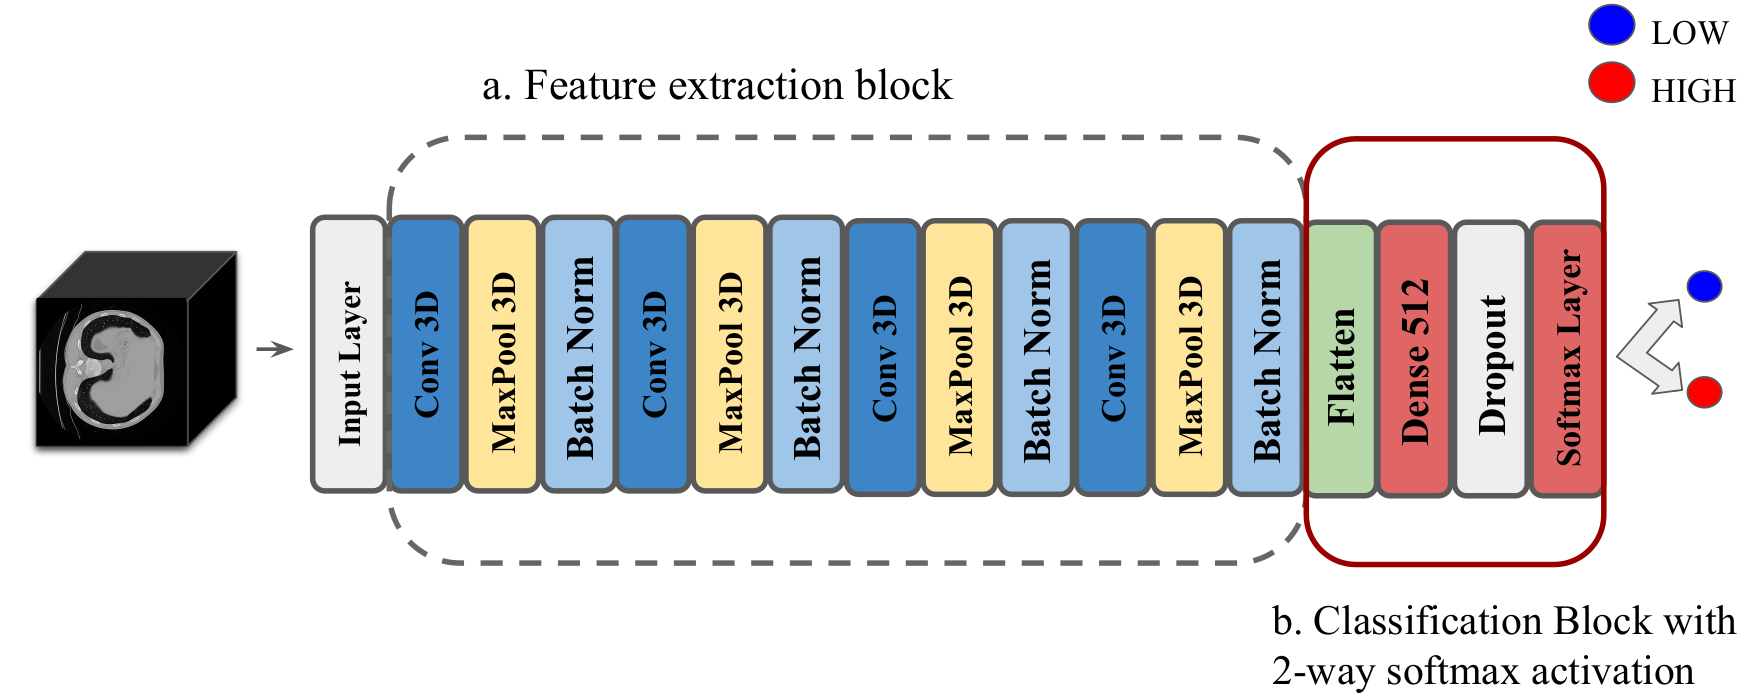
\includegraphics[width=0.8\linewidth]{images/network.pdf}
  \caption[The 3D CNN model]{The 3D CNN model. Image from \cite{Zunair2020}.}
  \label{fig:model}
\end{figure*}

For each PET scan image, a label based on the latest diagnosis will be assigned.
Since not all the scan sessions are associated with a psychiatric or
neurological test, each scan will be associated with the nearest test in time
(in both directions: either before the scan or after it). This first labeling
phase has been implemented in a Python 3.6+ script using Pandas version 1.2.4
\cite{Pandas-v1.2.4} and the results are provided in a simple CSV table.

\subsection{Dealing With Class Imbalance}
\label{sec:dealing-with-class}

After this first pre-processing step, a labeled dataset of PET scans was
obtained. It is made of 1217 negative samples and only 135 positive samples. It
is clear that, as 90\% of the samples are negative, this is a highly imbalanced
dataset. To deal with this issue, we opted for a combination of both a random
under-sampling of the negative class \cite{Japkowicz2002} and the application of
data augmentation techniques to the positive class. Details on both approaches
will be given in the subsequent paragraphs.

To perform the random under-sampling of the negative class, we first selected
all the negative scans of the same subjects that have positive scans: this would
allow the comparison between two images without any severe morphological
difference in the represented brains. This selection yielded a total of 23
images. Then, we randomly selected a total of 182 scans from the remaining
negative scans, reaching a total of 205 negative samples.

We then augmented the positive samples of about 50\% (thus obtaining a total of
205 images) through the means of randomly rotating and mirroring some images (as
executed by \cite{Altay2020}).


\section{Methods}
\label{sec:methods}

Since few works are currently available that rely on the classification of brain
amyloid PET scans, we have very few options for choosing the best model to
train. For this reason, we chose to test, as a future baseline, the relatively
simple 3D Convolutional Neural Network (3D CNN) model used by \cite{Zunair2020}
to recognize pneumonia in lungs' CT scans. The \cref{fig:model} represents the
structure of the model: a 17 layer 3D CNN which comprises four 3D convolutional
(CONV) layers with two layers consisting of 64 filters followed by 128 and 256
filters all with a kernel size of $3 \times 3 \times 3$ \cite{Zunair2020}. The
implementation was provided by the authors themselves
\cite{Zunair2020Implementation}, with some adaptations to use PET scans.

Before training the model, another pre-processing step was needed to resize the
images. PET scans are 3D images (i.e., a sequence of images that depict a
different slice of the brain along an axis) taken during a predefined time span.
For this reason, the first step is to decide how to treat the time coordinate in
the images. We chose to reduce the series of images in time to a single average
image, thus allowing us to treat the images as a typical MRI or CT image.

Each averaged PET scan, then, needs to be resized to a common size. To avoid
introducing upscaling artifacts, images' slices have been resized to the size of
128 voxels by 128 voxels, the minimum size available in the dataset. Similar
reasoning was applied to the choice of the number of slices to keep for each
image: to account for the diversity of scan settings and, thus, for the
diversity in the availability of slices, we chose to keep the 50 middle slices
as it's sure that they depict the subject brain (in a similar fashion to the
choice of middle slices in \cite{Altay2020}). Before resizing, the images have
been analyzed to identify a bounding box around the brain, in order to center
it: first, a heavily blurred (using a Gaussian blur of kernel size
$13 \times 13$ and $\sigma = 150$) version of the images have been segmented
using the Otsu threshold \cite{Otsu1979}, then a simple bounding box was
selected by detecting the ``high'' values in the images.

\section{Experiments}
\label{sec:experiments}

To evaluate the model, a simple stratified 10-fold cross-validation is used.
First, we split the dataset between a train set and a validation set (the latter
will be used to validate the final model), then we start the cross-validation
using the train set (that is further split into a smaller train set and a test
set). After the cross-validation, the model is re-trained on the entire original
train test, and it is validated on the validate test. Finally, the model is
re-trained on the entire available dataset. The execution of the experiment took
place on the Google Colaboratory
platform\footnote{\url{https://colab.research.google.com/}}, using a single GPU
(either Nvidia Tesla T4 or Nvidia Tesla P100, depending on their availability in
the cloud platform) for training. The \cref{fig:cv-results} represents the final
results of the stratified 10-fold cross-validation.

\begin{figure}[h]
  \centering
  \resizebox{\linewidth}{!}{%
    %% Creator: Matplotlib, PGF backend
%%
%% To include the figure in your LaTeX document, write
%%   \input{<filename>.pgf}
%%
%% Make sure the required packages are loaded in your preamble
%%   \usepackage{pgf}
%%
%% Figures using additional raster images can only be included by \input if
%% they are in the same directory as the main LaTeX file. For loading figures
%% from other directories you can use the `import` package
%%   \usepackage{import}
%%
%% and then include the figures with
%%   \import{<path to file>}{<filename>.pgf}
%%
%% Matplotlib used the following preamble
%%
\begingroup%
\makeatletter%
\begin{pgfpicture}%
\pgfpathrectangle{\pgfpointorigin}{\pgfqpoint{5.000000in}{2.500000in}}%
\pgfusepath{use as bounding box, clip}%
\begin{pgfscope}%
\pgfsetbuttcap%
\pgfsetmiterjoin%
\definecolor{currentfill}{rgb}{1.000000,1.000000,1.000000}%
\pgfsetfillcolor{currentfill}%
\pgfsetlinewidth{0.000000pt}%
\definecolor{currentstroke}{rgb}{1.000000,1.000000,1.000000}%
\pgfsetstrokecolor{currentstroke}%
\pgfsetdash{}{0pt}%
\pgfpathmoveto{\pgfqpoint{0.000000in}{0.000000in}}%
\pgfpathlineto{\pgfqpoint{5.000000in}{0.000000in}}%
\pgfpathlineto{\pgfqpoint{5.000000in}{2.500000in}}%
\pgfpathlineto{\pgfqpoint{0.000000in}{2.500000in}}%
\pgfpathclose%
\pgfusepath{fill}%
\end{pgfscope}%
\begin{pgfscope}%
\pgfsetbuttcap%
\pgfsetmiterjoin%
\definecolor{currentfill}{rgb}{1.000000,1.000000,1.000000}%
\pgfsetfillcolor{currentfill}%
\pgfsetlinewidth{0.000000pt}%
\definecolor{currentstroke}{rgb}{0.000000,0.000000,0.000000}%
\pgfsetstrokecolor{currentstroke}%
\pgfsetstrokeopacity{0.000000}%
\pgfsetdash{}{0pt}%
\pgfpathmoveto{\pgfqpoint{0.625000in}{0.275000in}}%
\pgfpathlineto{\pgfqpoint{2.386364in}{0.275000in}}%
\pgfpathlineto{\pgfqpoint{2.386364in}{2.200000in}}%
\pgfpathlineto{\pgfqpoint{0.625000in}{2.200000in}}%
\pgfpathclose%
\pgfusepath{fill}%
\end{pgfscope}%
\begin{pgfscope}%
\pgfpathrectangle{\pgfqpoint{0.625000in}{0.275000in}}{\pgfqpoint{1.761364in}{1.925000in}}%
\pgfusepath{clip}%
\pgfsetbuttcap%
\pgfsetmiterjoin%
\definecolor{currentfill}{rgb}{0.121569,0.466667,0.705882}%
\pgfsetfillcolor{currentfill}%
\pgfsetlinewidth{0.000000pt}%
\definecolor{currentstroke}{rgb}{0.000000,0.000000,0.000000}%
\pgfsetstrokecolor{currentstroke}%
\pgfsetstrokeopacity{0.000000}%
\pgfsetdash{}{0pt}%
\pgfpathmoveto{\pgfqpoint{0.705062in}{-0.275000in}}%
\pgfpathlineto{\pgfqpoint{1.416724in}{-0.275000in}}%
\pgfpathlineto{\pgfqpoint{1.416724in}{1.029639in}}%
\pgfpathlineto{\pgfqpoint{0.705062in}{1.029639in}}%
\pgfpathclose%
\pgfusepath{fill}%
\end{pgfscope}%
\begin{pgfscope}%
\pgfpathrectangle{\pgfqpoint{0.625000in}{0.275000in}}{\pgfqpoint{1.761364in}{1.925000in}}%
\pgfusepath{clip}%
\pgfsetbuttcap%
\pgfsetmiterjoin%
\definecolor{currentfill}{rgb}{0.121569,0.466667,0.705882}%
\pgfsetfillcolor{currentfill}%
\pgfsetlinewidth{0.000000pt}%
\definecolor{currentstroke}{rgb}{0.000000,0.000000,0.000000}%
\pgfsetstrokecolor{currentstroke}%
\pgfsetstrokeopacity{0.000000}%
\pgfsetdash{}{0pt}%
\pgfpathmoveto{\pgfqpoint{1.594640in}{-0.275000in}}%
\pgfpathlineto{\pgfqpoint{2.306302in}{-0.275000in}}%
\pgfpathlineto{\pgfqpoint{2.306302in}{1.830469in}}%
\pgfpathlineto{\pgfqpoint{1.594640in}{1.830469in}}%
\pgfpathclose%
\pgfusepath{fill}%
\end{pgfscope}%
\begin{pgfscope}%
\pgfsetbuttcap%
\pgfsetroundjoin%
\definecolor{currentfill}{rgb}{0.000000,0.000000,0.000000}%
\pgfsetfillcolor{currentfill}%
\pgfsetlinewidth{0.803000pt}%
\definecolor{currentstroke}{rgb}{0.000000,0.000000,0.000000}%
\pgfsetstrokecolor{currentstroke}%
\pgfsetdash{}{0pt}%
\pgfsys@defobject{currentmarker}{\pgfqpoint{0.000000in}{-0.048611in}}{\pgfqpoint{0.000000in}{0.000000in}}{%
\pgfpathmoveto{\pgfqpoint{0.000000in}{0.000000in}}%
\pgfpathlineto{\pgfqpoint{0.000000in}{-0.048611in}}%
\pgfusepath{stroke,fill}%
}%
\begin{pgfscope}%
\pgfsys@transformshift{1.060893in}{0.275000in}%
\pgfsys@useobject{currentmarker}{}%
\end{pgfscope}%
\end{pgfscope}%
\begin{pgfscope}%
\definecolor{textcolor}{rgb}{0.000000,0.000000,0.000000}%
\pgfsetstrokecolor{textcolor}%
\pgfsetfillcolor{textcolor}%
\pgftext[x=1.060893in,y=0.177778in,,top]{\color{textcolor}\rmfamily\fontsize{10.000000}{12.000000}\selectfont loss}%
\end{pgfscope}%
\begin{pgfscope}%
\pgfsetbuttcap%
\pgfsetroundjoin%
\definecolor{currentfill}{rgb}{0.000000,0.000000,0.000000}%
\pgfsetfillcolor{currentfill}%
\pgfsetlinewidth{0.803000pt}%
\definecolor{currentstroke}{rgb}{0.000000,0.000000,0.000000}%
\pgfsetstrokecolor{currentstroke}%
\pgfsetdash{}{0pt}%
\pgfsys@defobject{currentmarker}{\pgfqpoint{0.000000in}{-0.048611in}}{\pgfqpoint{0.000000in}{0.000000in}}{%
\pgfpathmoveto{\pgfqpoint{0.000000in}{0.000000in}}%
\pgfpathlineto{\pgfqpoint{0.000000in}{-0.048611in}}%
\pgfusepath{stroke,fill}%
}%
\begin{pgfscope}%
\pgfsys@transformshift{1.950471in}{0.275000in}%
\pgfsys@useobject{currentmarker}{}%
\end{pgfscope}%
\end{pgfscope}%
\begin{pgfscope}%
\definecolor{textcolor}{rgb}{0.000000,0.000000,0.000000}%
\pgfsetstrokecolor{textcolor}%
\pgfsetfillcolor{textcolor}%
\pgftext[x=1.950471in,y=0.177778in,,top]{\color{textcolor}\rmfamily\fontsize{10.000000}{12.000000}\selectfont accuracy}%
\end{pgfscope}%
\begin{pgfscope}%
\pgfsetbuttcap%
\pgfsetroundjoin%
\definecolor{currentfill}{rgb}{0.000000,0.000000,0.000000}%
\pgfsetfillcolor{currentfill}%
\pgfsetlinewidth{0.803000pt}%
\definecolor{currentstroke}{rgb}{0.000000,0.000000,0.000000}%
\pgfsetstrokecolor{currentstroke}%
\pgfsetdash{}{0pt}%
\pgfsys@defobject{currentmarker}{\pgfqpoint{-0.048611in}{0.000000in}}{\pgfqpoint{-0.000000in}{0.000000in}}{%
\pgfpathmoveto{\pgfqpoint{-0.000000in}{0.000000in}}%
\pgfpathlineto{\pgfqpoint{-0.048611in}{0.000000in}}%
\pgfusepath{stroke,fill}%
}%
\begin{pgfscope}%
\pgfsys@transformshift{0.625000in}{0.275000in}%
\pgfsys@useobject{currentmarker}{}%
\end{pgfscope}%
\end{pgfscope}%
\begin{pgfscope}%
\definecolor{textcolor}{rgb}{0.000000,0.000000,0.000000}%
\pgfsetstrokecolor{textcolor}%
\pgfsetfillcolor{textcolor}%
\pgftext[x=0.350308in, y=0.226775in, left, base]{\color{textcolor}\rmfamily\fontsize{10.000000}{12.000000}\selectfont \(\displaystyle {0.2}\)}%
\end{pgfscope}%
\begin{pgfscope}%
\pgfsetbuttcap%
\pgfsetroundjoin%
\definecolor{currentfill}{rgb}{0.000000,0.000000,0.000000}%
\pgfsetfillcolor{currentfill}%
\pgfsetlinewidth{0.803000pt}%
\definecolor{currentstroke}{rgb}{0.000000,0.000000,0.000000}%
\pgfsetstrokecolor{currentstroke}%
\pgfsetdash{}{0pt}%
\pgfsys@defobject{currentmarker}{\pgfqpoint{-0.048611in}{0.000000in}}{\pgfqpoint{-0.000000in}{0.000000in}}{%
\pgfpathmoveto{\pgfqpoint{-0.000000in}{0.000000in}}%
\pgfpathlineto{\pgfqpoint{-0.048611in}{0.000000in}}%
\pgfusepath{stroke,fill}%
}%
\begin{pgfscope}%
\pgfsys@transformshift{0.625000in}{0.825000in}%
\pgfsys@useobject{currentmarker}{}%
\end{pgfscope}%
\end{pgfscope}%
\begin{pgfscope}%
\definecolor{textcolor}{rgb}{0.000000,0.000000,0.000000}%
\pgfsetstrokecolor{textcolor}%
\pgfsetfillcolor{textcolor}%
\pgftext[x=0.350308in, y=0.776775in, left, base]{\color{textcolor}\rmfamily\fontsize{10.000000}{12.000000}\selectfont \(\displaystyle {0.4}\)}%
\end{pgfscope}%
\begin{pgfscope}%
\pgfsetbuttcap%
\pgfsetroundjoin%
\definecolor{currentfill}{rgb}{0.000000,0.000000,0.000000}%
\pgfsetfillcolor{currentfill}%
\pgfsetlinewidth{0.803000pt}%
\definecolor{currentstroke}{rgb}{0.000000,0.000000,0.000000}%
\pgfsetstrokecolor{currentstroke}%
\pgfsetdash{}{0pt}%
\pgfsys@defobject{currentmarker}{\pgfqpoint{-0.048611in}{0.000000in}}{\pgfqpoint{-0.000000in}{0.000000in}}{%
\pgfpathmoveto{\pgfqpoint{-0.000000in}{0.000000in}}%
\pgfpathlineto{\pgfqpoint{-0.048611in}{0.000000in}}%
\pgfusepath{stroke,fill}%
}%
\begin{pgfscope}%
\pgfsys@transformshift{0.625000in}{1.375000in}%
\pgfsys@useobject{currentmarker}{}%
\end{pgfscope}%
\end{pgfscope}%
\begin{pgfscope}%
\definecolor{textcolor}{rgb}{0.000000,0.000000,0.000000}%
\pgfsetstrokecolor{textcolor}%
\pgfsetfillcolor{textcolor}%
\pgftext[x=0.350308in, y=1.326775in, left, base]{\color{textcolor}\rmfamily\fontsize{10.000000}{12.000000}\selectfont \(\displaystyle {0.6}\)}%
\end{pgfscope}%
\begin{pgfscope}%
\pgfsetbuttcap%
\pgfsetroundjoin%
\definecolor{currentfill}{rgb}{0.000000,0.000000,0.000000}%
\pgfsetfillcolor{currentfill}%
\pgfsetlinewidth{0.803000pt}%
\definecolor{currentstroke}{rgb}{0.000000,0.000000,0.000000}%
\pgfsetstrokecolor{currentstroke}%
\pgfsetdash{}{0pt}%
\pgfsys@defobject{currentmarker}{\pgfqpoint{-0.048611in}{0.000000in}}{\pgfqpoint{-0.000000in}{0.000000in}}{%
\pgfpathmoveto{\pgfqpoint{-0.000000in}{0.000000in}}%
\pgfpathlineto{\pgfqpoint{-0.048611in}{0.000000in}}%
\pgfusepath{stroke,fill}%
}%
\begin{pgfscope}%
\pgfsys@transformshift{0.625000in}{1.925000in}%
\pgfsys@useobject{currentmarker}{}%
\end{pgfscope}%
\end{pgfscope}%
\begin{pgfscope}%
\definecolor{textcolor}{rgb}{0.000000,0.000000,0.000000}%
\pgfsetstrokecolor{textcolor}%
\pgfsetfillcolor{textcolor}%
\pgftext[x=0.350308in, y=1.876775in, left, base]{\color{textcolor}\rmfamily\fontsize{10.000000}{12.000000}\selectfont \(\displaystyle {0.8}\)}%
\end{pgfscope}%
\begin{pgfscope}%
\pgfpathrectangle{\pgfqpoint{0.625000in}{0.275000in}}{\pgfqpoint{1.761364in}{1.925000in}}%
\pgfusepath{clip}%
\pgfsetbuttcap%
\pgfsetroundjoin%
\pgfsetlinewidth{1.505625pt}%
\definecolor{currentstroke}{rgb}{0.000000,0.000000,0.000000}%
\pgfsetstrokecolor{currentstroke}%
\pgfsetdash{}{0pt}%
\pgfpathmoveto{\pgfqpoint{1.060893in}{0.720479in}}%
\pgfpathlineto{\pgfqpoint{1.060893in}{1.338800in}}%
\pgfusepath{stroke}%
\end{pgfscope}%
\begin{pgfscope}%
\pgfpathrectangle{\pgfqpoint{0.625000in}{0.275000in}}{\pgfqpoint{1.761364in}{1.925000in}}%
\pgfusepath{clip}%
\pgfsetbuttcap%
\pgfsetroundjoin%
\pgfsetlinewidth{1.505625pt}%
\definecolor{currentstroke}{rgb}{0.000000,0.000000,0.000000}%
\pgfsetstrokecolor{currentstroke}%
\pgfsetdash{}{0pt}%
\pgfpathmoveto{\pgfqpoint{1.950471in}{1.563509in}}%
\pgfpathlineto{\pgfqpoint{1.950471in}{2.097429in}}%
\pgfusepath{stroke}%
\end{pgfscope}%
\begin{pgfscope}%
\pgfpathrectangle{\pgfqpoint{0.625000in}{0.275000in}}{\pgfqpoint{1.761364in}{1.925000in}}%
\pgfusepath{clip}%
\pgfsetbuttcap%
\pgfsetroundjoin%
\definecolor{currentfill}{rgb}{0.000000,0.000000,0.000000}%
\pgfsetfillcolor{currentfill}%
\pgfsetlinewidth{1.003750pt}%
\definecolor{currentstroke}{rgb}{0.000000,0.000000,0.000000}%
\pgfsetstrokecolor{currentstroke}%
\pgfsetdash{}{0pt}%
\pgfsys@defobject{currentmarker}{\pgfqpoint{-0.041667in}{-0.000000in}}{\pgfqpoint{0.041667in}{0.000000in}}{%
\pgfpathmoveto{\pgfqpoint{0.041667in}{-0.000000in}}%
\pgfpathlineto{\pgfqpoint{-0.041667in}{0.000000in}}%
\pgfusepath{stroke,fill}%
}%
\begin{pgfscope}%
\pgfsys@transformshift{1.060893in}{0.720479in}%
\pgfsys@useobject{currentmarker}{}%
\end{pgfscope}%
\begin{pgfscope}%
\pgfsys@transformshift{1.950471in}{1.563509in}%
\pgfsys@useobject{currentmarker}{}%
\end{pgfscope}%
\end{pgfscope}%
\begin{pgfscope}%
\pgfpathrectangle{\pgfqpoint{0.625000in}{0.275000in}}{\pgfqpoint{1.761364in}{1.925000in}}%
\pgfusepath{clip}%
\pgfsetbuttcap%
\pgfsetroundjoin%
\definecolor{currentfill}{rgb}{0.000000,0.000000,0.000000}%
\pgfsetfillcolor{currentfill}%
\pgfsetlinewidth{1.003750pt}%
\definecolor{currentstroke}{rgb}{0.000000,0.000000,0.000000}%
\pgfsetstrokecolor{currentstroke}%
\pgfsetdash{}{0pt}%
\pgfsys@defobject{currentmarker}{\pgfqpoint{-0.041667in}{-0.000000in}}{\pgfqpoint{0.041667in}{0.000000in}}{%
\pgfpathmoveto{\pgfqpoint{0.041667in}{-0.000000in}}%
\pgfpathlineto{\pgfqpoint{-0.041667in}{0.000000in}}%
\pgfusepath{stroke,fill}%
}%
\begin{pgfscope}%
\pgfsys@transformshift{1.060893in}{1.338800in}%
\pgfsys@useobject{currentmarker}{}%
\end{pgfscope}%
\begin{pgfscope}%
\pgfsys@transformshift{1.950471in}{2.097429in}%
\pgfsys@useobject{currentmarker}{}%
\end{pgfscope}%
\end{pgfscope}%
\begin{pgfscope}%
\pgfsetrectcap%
\pgfsetmiterjoin%
\pgfsetlinewidth{0.803000pt}%
\definecolor{currentstroke}{rgb}{0.000000,0.000000,0.000000}%
\pgfsetstrokecolor{currentstroke}%
\pgfsetdash{}{0pt}%
\pgfpathmoveto{\pgfqpoint{0.625000in}{0.275000in}}%
\pgfpathlineto{\pgfqpoint{0.625000in}{2.200000in}}%
\pgfusepath{stroke}%
\end{pgfscope}%
\begin{pgfscope}%
\pgfsetrectcap%
\pgfsetmiterjoin%
\pgfsetlinewidth{0.803000pt}%
\definecolor{currentstroke}{rgb}{0.000000,0.000000,0.000000}%
\pgfsetstrokecolor{currentstroke}%
\pgfsetdash{}{0pt}%
\pgfpathmoveto{\pgfqpoint{2.386364in}{0.275000in}}%
\pgfpathlineto{\pgfqpoint{2.386364in}{2.200000in}}%
\pgfusepath{stroke}%
\end{pgfscope}%
\begin{pgfscope}%
\pgfsetrectcap%
\pgfsetmiterjoin%
\pgfsetlinewidth{0.803000pt}%
\definecolor{currentstroke}{rgb}{0.000000,0.000000,0.000000}%
\pgfsetstrokecolor{currentstroke}%
\pgfsetdash{}{0pt}%
\pgfpathmoveto{\pgfqpoint{0.625000in}{0.275000in}}%
\pgfpathlineto{\pgfqpoint{2.386364in}{0.275000in}}%
\pgfusepath{stroke}%
\end{pgfscope}%
\begin{pgfscope}%
\pgfsetrectcap%
\pgfsetmiterjoin%
\pgfsetlinewidth{0.803000pt}%
\definecolor{currentstroke}{rgb}{0.000000,0.000000,0.000000}%
\pgfsetstrokecolor{currentstroke}%
\pgfsetdash{}{0pt}%
\pgfpathmoveto{\pgfqpoint{0.625000in}{2.200000in}}%
\pgfpathlineto{\pgfqpoint{2.386364in}{2.200000in}}%
\pgfusepath{stroke}%
\end{pgfscope}%
\begin{pgfscope}%
\pgfsetbuttcap%
\pgfsetmiterjoin%
\definecolor{currentfill}{rgb}{1.000000,1.000000,1.000000}%
\pgfsetfillcolor{currentfill}%
\pgfsetlinewidth{0.000000pt}%
\definecolor{currentstroke}{rgb}{0.000000,0.000000,0.000000}%
\pgfsetstrokecolor{currentstroke}%
\pgfsetstrokeopacity{0.000000}%
\pgfsetdash{}{0pt}%
\pgfpathmoveto{\pgfqpoint{2.738636in}{0.275000in}}%
\pgfpathlineto{\pgfqpoint{4.500000in}{0.275000in}}%
\pgfpathlineto{\pgfqpoint{4.500000in}{2.200000in}}%
\pgfpathlineto{\pgfqpoint{2.738636in}{2.200000in}}%
\pgfpathclose%
\pgfusepath{fill}%
\end{pgfscope}%
\begin{pgfscope}%
\pgfsetbuttcap%
\pgfsetroundjoin%
\definecolor{currentfill}{rgb}{0.000000,0.000000,0.000000}%
\pgfsetfillcolor{currentfill}%
\pgfsetlinewidth{0.803000pt}%
\definecolor{currentstroke}{rgb}{0.000000,0.000000,0.000000}%
\pgfsetstrokecolor{currentstroke}%
\pgfsetdash{}{0pt}%
\pgfsys@defobject{currentmarker}{\pgfqpoint{0.000000in}{-0.048611in}}{\pgfqpoint{0.000000in}{0.000000in}}{%
\pgfpathmoveto{\pgfqpoint{0.000000in}{0.000000in}}%
\pgfpathlineto{\pgfqpoint{0.000000in}{-0.048611in}}%
\pgfusepath{stroke,fill}%
}%
\begin{pgfscope}%
\pgfsys@transformshift{3.178977in}{0.275000in}%
\pgfsys@useobject{currentmarker}{}%
\end{pgfscope}%
\end{pgfscope}%
\begin{pgfscope}%
\definecolor{textcolor}{rgb}{0.000000,0.000000,0.000000}%
\pgfsetstrokecolor{textcolor}%
\pgfsetfillcolor{textcolor}%
\pgftext[x=3.178977in,y=0.177778in,,top]{\color{textcolor}\rmfamily\fontsize{10.000000}{12.000000}\selectfont loss}%
\end{pgfscope}%
\begin{pgfscope}%
\pgfsetbuttcap%
\pgfsetroundjoin%
\definecolor{currentfill}{rgb}{0.000000,0.000000,0.000000}%
\pgfsetfillcolor{currentfill}%
\pgfsetlinewidth{0.803000pt}%
\definecolor{currentstroke}{rgb}{0.000000,0.000000,0.000000}%
\pgfsetstrokecolor{currentstroke}%
\pgfsetdash{}{0pt}%
\pgfsys@defobject{currentmarker}{\pgfqpoint{0.000000in}{-0.048611in}}{\pgfqpoint{0.000000in}{0.000000in}}{%
\pgfpathmoveto{\pgfqpoint{0.000000in}{0.000000in}}%
\pgfpathlineto{\pgfqpoint{0.000000in}{-0.048611in}}%
\pgfusepath{stroke,fill}%
}%
\begin{pgfscope}%
\pgfsys@transformshift{4.059659in}{0.275000in}%
\pgfsys@useobject{currentmarker}{}%
\end{pgfscope}%
\end{pgfscope}%
\begin{pgfscope}%
\definecolor{textcolor}{rgb}{0.000000,0.000000,0.000000}%
\pgfsetstrokecolor{textcolor}%
\pgfsetfillcolor{textcolor}%
\pgftext[x=4.059659in,y=0.177778in,,top]{\color{textcolor}\rmfamily\fontsize{10.000000}{12.000000}\selectfont accuracy}%
\end{pgfscope}%
\begin{pgfscope}%
\pgfsetbuttcap%
\pgfsetroundjoin%
\definecolor{currentfill}{rgb}{0.000000,0.000000,0.000000}%
\pgfsetfillcolor{currentfill}%
\pgfsetlinewidth{0.803000pt}%
\definecolor{currentstroke}{rgb}{0.000000,0.000000,0.000000}%
\pgfsetstrokecolor{currentstroke}%
\pgfsetdash{}{0pt}%
\pgfsys@defobject{currentmarker}{\pgfqpoint{-0.048611in}{0.000000in}}{\pgfqpoint{-0.000000in}{0.000000in}}{%
\pgfpathmoveto{\pgfqpoint{-0.000000in}{0.000000in}}%
\pgfpathlineto{\pgfqpoint{-0.048611in}{0.000000in}}%
\pgfusepath{stroke,fill}%
}%
\begin{pgfscope}%
\pgfsys@transformshift{2.738636in}{0.784397in}%
\pgfsys@useobject{currentmarker}{}%
\end{pgfscope}%
\end{pgfscope}%
\begin{pgfscope}%
\definecolor{textcolor}{rgb}{0.000000,0.000000,0.000000}%
\pgfsetstrokecolor{textcolor}%
\pgfsetfillcolor{textcolor}%
\pgftext[x=2.463944in, y=0.736172in, left, base]{\color{textcolor}\rmfamily\fontsize{10.000000}{12.000000}\selectfont \(\displaystyle {0.4}\)}%
\end{pgfscope}%
\begin{pgfscope}%
\pgfsetbuttcap%
\pgfsetroundjoin%
\definecolor{currentfill}{rgb}{0.000000,0.000000,0.000000}%
\pgfsetfillcolor{currentfill}%
\pgfsetlinewidth{0.803000pt}%
\definecolor{currentstroke}{rgb}{0.000000,0.000000,0.000000}%
\pgfsetstrokecolor{currentstroke}%
\pgfsetdash{}{0pt}%
\pgfsys@defobject{currentmarker}{\pgfqpoint{-0.048611in}{0.000000in}}{\pgfqpoint{-0.000000in}{0.000000in}}{%
\pgfpathmoveto{\pgfqpoint{-0.000000in}{0.000000in}}%
\pgfpathlineto{\pgfqpoint{-0.048611in}{0.000000in}}%
\pgfusepath{stroke,fill}%
}%
\begin{pgfscope}%
\pgfsys@transformshift{2.738636in}{1.343598in}%
\pgfsys@useobject{currentmarker}{}%
\end{pgfscope}%
\end{pgfscope}%
\begin{pgfscope}%
\definecolor{textcolor}{rgb}{0.000000,0.000000,0.000000}%
\pgfsetstrokecolor{textcolor}%
\pgfsetfillcolor{textcolor}%
\pgftext[x=2.463944in, y=1.295373in, left, base]{\color{textcolor}\rmfamily\fontsize{10.000000}{12.000000}\selectfont \(\displaystyle {0.6}\)}%
\end{pgfscope}%
\begin{pgfscope}%
\pgfsetbuttcap%
\pgfsetroundjoin%
\definecolor{currentfill}{rgb}{0.000000,0.000000,0.000000}%
\pgfsetfillcolor{currentfill}%
\pgfsetlinewidth{0.803000pt}%
\definecolor{currentstroke}{rgb}{0.000000,0.000000,0.000000}%
\pgfsetstrokecolor{currentstroke}%
\pgfsetdash{}{0pt}%
\pgfsys@defobject{currentmarker}{\pgfqpoint{-0.048611in}{0.000000in}}{\pgfqpoint{-0.000000in}{0.000000in}}{%
\pgfpathmoveto{\pgfqpoint{-0.000000in}{0.000000in}}%
\pgfpathlineto{\pgfqpoint{-0.048611in}{0.000000in}}%
\pgfusepath{stroke,fill}%
}%
\begin{pgfscope}%
\pgfsys@transformshift{2.738636in}{1.902800in}%
\pgfsys@useobject{currentmarker}{}%
\end{pgfscope}%
\end{pgfscope}%
\begin{pgfscope}%
\definecolor{textcolor}{rgb}{0.000000,0.000000,0.000000}%
\pgfsetstrokecolor{textcolor}%
\pgfsetfillcolor{textcolor}%
\pgftext[x=2.463944in, y=1.854574in, left, base]{\color{textcolor}\rmfamily\fontsize{10.000000}{12.000000}\selectfont \(\displaystyle {0.8}\)}%
\end{pgfscope}%
\begin{pgfscope}%
\pgfpathrectangle{\pgfqpoint{2.738636in}{0.275000in}}{\pgfqpoint{1.761364in}{1.925000in}}%
\pgfusepath{clip}%
\pgfsetrectcap%
\pgfsetroundjoin%
\pgfsetlinewidth{1.003750pt}%
\definecolor{currentstroke}{rgb}{0.000000,0.000000,0.000000}%
\pgfsetstrokecolor{currentstroke}%
\pgfsetdash{}{0pt}%
\pgfpathmoveto{\pgfqpoint{2.958807in}{0.820410in}}%
\pgfpathlineto{\pgfqpoint{3.399148in}{0.820410in}}%
\pgfpathlineto{\pgfqpoint{3.399148in}{1.206541in}}%
\pgfpathlineto{\pgfqpoint{2.958807in}{1.206541in}}%
\pgfpathlineto{\pgfqpoint{2.958807in}{0.820410in}}%
\pgfusepath{stroke}%
\end{pgfscope}%
\begin{pgfscope}%
\pgfpathrectangle{\pgfqpoint{2.738636in}{0.275000in}}{\pgfqpoint{1.761364in}{1.925000in}}%
\pgfusepath{clip}%
\pgfsetrectcap%
\pgfsetroundjoin%
\pgfsetlinewidth{1.003750pt}%
\definecolor{currentstroke}{rgb}{0.000000,0.000000,0.000000}%
\pgfsetstrokecolor{currentstroke}%
\pgfsetdash{}{0pt}%
\pgfpathmoveto{\pgfqpoint{3.178977in}{0.820410in}}%
\pgfpathlineto{\pgfqpoint{3.178977in}{0.362500in}}%
\pgfusepath{stroke}%
\end{pgfscope}%
\begin{pgfscope}%
\pgfpathrectangle{\pgfqpoint{2.738636in}{0.275000in}}{\pgfqpoint{1.761364in}{1.925000in}}%
\pgfusepath{clip}%
\pgfsetrectcap%
\pgfsetroundjoin%
\pgfsetlinewidth{1.003750pt}%
\definecolor{currentstroke}{rgb}{0.000000,0.000000,0.000000}%
\pgfsetstrokecolor{currentstroke}%
\pgfsetdash{}{0pt}%
\pgfpathmoveto{\pgfqpoint{3.178977in}{1.206541in}}%
\pgfpathlineto{\pgfqpoint{3.178977in}{1.566490in}}%
\pgfusepath{stroke}%
\end{pgfscope}%
\begin{pgfscope}%
\pgfpathrectangle{\pgfqpoint{2.738636in}{0.275000in}}{\pgfqpoint{1.761364in}{1.925000in}}%
\pgfusepath{clip}%
\pgfsetrectcap%
\pgfsetroundjoin%
\pgfsetlinewidth{1.003750pt}%
\definecolor{currentstroke}{rgb}{0.000000,0.000000,0.000000}%
\pgfsetstrokecolor{currentstroke}%
\pgfsetdash{}{0pt}%
\pgfpathmoveto{\pgfqpoint{3.068892in}{0.362500in}}%
\pgfpathlineto{\pgfqpoint{3.289062in}{0.362500in}}%
\pgfusepath{stroke}%
\end{pgfscope}%
\begin{pgfscope}%
\pgfpathrectangle{\pgfqpoint{2.738636in}{0.275000in}}{\pgfqpoint{1.761364in}{1.925000in}}%
\pgfusepath{clip}%
\pgfsetrectcap%
\pgfsetroundjoin%
\pgfsetlinewidth{1.003750pt}%
\definecolor{currentstroke}{rgb}{0.000000,0.000000,0.000000}%
\pgfsetstrokecolor{currentstroke}%
\pgfsetdash{}{0pt}%
\pgfpathmoveto{\pgfqpoint{3.068892in}{1.566490in}}%
\pgfpathlineto{\pgfqpoint{3.289062in}{1.566490in}}%
\pgfusepath{stroke}%
\end{pgfscope}%
\begin{pgfscope}%
\pgfpathrectangle{\pgfqpoint{2.738636in}{0.275000in}}{\pgfqpoint{1.761364in}{1.925000in}}%
\pgfusepath{clip}%
\pgfsetrectcap%
\pgfsetroundjoin%
\pgfsetlinewidth{1.003750pt}%
\definecolor{currentstroke}{rgb}{0.000000,0.000000,0.000000}%
\pgfsetstrokecolor{currentstroke}%
\pgfsetdash{}{0pt}%
\pgfpathmoveto{\pgfqpoint{3.839489in}{1.675624in}}%
\pgfpathlineto{\pgfqpoint{4.279830in}{1.675624in}}%
\pgfpathlineto{\pgfqpoint{4.279830in}{2.003281in}}%
\pgfpathlineto{\pgfqpoint{3.839489in}{2.003281in}}%
\pgfpathlineto{\pgfqpoint{3.839489in}{1.675624in}}%
\pgfusepath{stroke}%
\end{pgfscope}%
\begin{pgfscope}%
\pgfpathrectangle{\pgfqpoint{2.738636in}{0.275000in}}{\pgfqpoint{1.761364in}{1.925000in}}%
\pgfusepath{clip}%
\pgfsetrectcap%
\pgfsetroundjoin%
\pgfsetlinewidth{1.003750pt}%
\definecolor{currentstroke}{rgb}{0.000000,0.000000,0.000000}%
\pgfsetstrokecolor{currentstroke}%
\pgfsetdash{}{0pt}%
\pgfpathmoveto{\pgfqpoint{4.059659in}{1.675624in}}%
\pgfpathlineto{\pgfqpoint{4.059659in}{1.675624in}}%
\pgfusepath{stroke}%
\end{pgfscope}%
\begin{pgfscope}%
\pgfpathrectangle{\pgfqpoint{2.738636in}{0.275000in}}{\pgfqpoint{1.761364in}{1.925000in}}%
\pgfusepath{clip}%
\pgfsetrectcap%
\pgfsetroundjoin%
\pgfsetlinewidth{1.003750pt}%
\definecolor{currentstroke}{rgb}{0.000000,0.000000,0.000000}%
\pgfsetstrokecolor{currentstroke}%
\pgfsetdash{}{0pt}%
\pgfpathmoveto{\pgfqpoint{4.059659in}{2.003281in}}%
\pgfpathlineto{\pgfqpoint{4.059659in}{2.112500in}}%
\pgfusepath{stroke}%
\end{pgfscope}%
\begin{pgfscope}%
\pgfpathrectangle{\pgfqpoint{2.738636in}{0.275000in}}{\pgfqpoint{1.761364in}{1.925000in}}%
\pgfusepath{clip}%
\pgfsetrectcap%
\pgfsetroundjoin%
\pgfsetlinewidth{1.003750pt}%
\definecolor{currentstroke}{rgb}{0.000000,0.000000,0.000000}%
\pgfsetstrokecolor{currentstroke}%
\pgfsetdash{}{0pt}%
\pgfpathmoveto{\pgfqpoint{3.949574in}{1.675624in}}%
\pgfpathlineto{\pgfqpoint{4.169744in}{1.675624in}}%
\pgfusepath{stroke}%
\end{pgfscope}%
\begin{pgfscope}%
\pgfpathrectangle{\pgfqpoint{2.738636in}{0.275000in}}{\pgfqpoint{1.761364in}{1.925000in}}%
\pgfusepath{clip}%
\pgfsetrectcap%
\pgfsetroundjoin%
\pgfsetlinewidth{1.003750pt}%
\definecolor{currentstroke}{rgb}{0.000000,0.000000,0.000000}%
\pgfsetstrokecolor{currentstroke}%
\pgfsetdash{}{0pt}%
\pgfpathmoveto{\pgfqpoint{3.949574in}{2.112500in}}%
\pgfpathlineto{\pgfqpoint{4.169744in}{2.112500in}}%
\pgfusepath{stroke}%
\end{pgfscope}%
\begin{pgfscope}%
\pgfpathrectangle{\pgfqpoint{2.738636in}{0.275000in}}{\pgfqpoint{1.761364in}{1.925000in}}%
\pgfusepath{clip}%
\pgfsetbuttcap%
\pgfsetroundjoin%
\definecolor{currentfill}{rgb}{0.000000,0.000000,0.000000}%
\pgfsetfillcolor{currentfill}%
\pgfsetfillopacity{0.000000}%
\pgfsetlinewidth{1.003750pt}%
\definecolor{currentstroke}{rgb}{0.000000,0.000000,0.000000}%
\pgfsetstrokecolor{currentstroke}%
\pgfsetdash{}{0pt}%
\pgfsys@defobject{currentmarker}{\pgfqpoint{-0.041667in}{-0.041667in}}{\pgfqpoint{0.041667in}{0.041667in}}{%
\pgfpathmoveto{\pgfqpoint{0.000000in}{-0.041667in}}%
\pgfpathcurveto{\pgfqpoint{0.011050in}{-0.041667in}}{\pgfqpoint{0.021649in}{-0.037276in}}{\pgfqpoint{0.029463in}{-0.029463in}}%
\pgfpathcurveto{\pgfqpoint{0.037276in}{-0.021649in}}{\pgfqpoint{0.041667in}{-0.011050in}}{\pgfqpoint{0.041667in}{0.000000in}}%
\pgfpathcurveto{\pgfqpoint{0.041667in}{0.011050in}}{\pgfqpoint{0.037276in}{0.021649in}}{\pgfqpoint{0.029463in}{0.029463in}}%
\pgfpathcurveto{\pgfqpoint{0.021649in}{0.037276in}}{\pgfqpoint{0.011050in}{0.041667in}}{\pgfqpoint{0.000000in}{0.041667in}}%
\pgfpathcurveto{\pgfqpoint{-0.011050in}{0.041667in}}{\pgfqpoint{-0.021649in}{0.037276in}}{\pgfqpoint{-0.029463in}{0.029463in}}%
\pgfpathcurveto{\pgfqpoint{-0.037276in}{0.021649in}}{\pgfqpoint{-0.041667in}{0.011050in}}{\pgfqpoint{-0.041667in}{0.000000in}}%
\pgfpathcurveto{\pgfqpoint{-0.041667in}{-0.011050in}}{\pgfqpoint{-0.037276in}{-0.021649in}}{\pgfqpoint{-0.029463in}{-0.029463in}}%
\pgfpathcurveto{\pgfqpoint{-0.021649in}{-0.037276in}}{\pgfqpoint{-0.011050in}{-0.041667in}}{\pgfqpoint{0.000000in}{-0.041667in}}%
\pgfpathclose%
\pgfusepath{stroke,fill}%
}%
\begin{pgfscope}%
\pgfsys@transformshift{4.059659in}{1.151373in}%
\pgfsys@useobject{currentmarker}{}%
\end{pgfscope}%
\end{pgfscope}%
\begin{pgfscope}%
\pgfpathrectangle{\pgfqpoint{2.738636in}{0.275000in}}{\pgfqpoint{1.761364in}{1.925000in}}%
\pgfusepath{clip}%
\pgfsetrectcap%
\pgfsetroundjoin%
\pgfsetlinewidth{1.003750pt}%
\definecolor{currentstroke}{rgb}{1.000000,0.498039,0.054902}%
\pgfsetstrokecolor{currentstroke}%
\pgfsetdash{}{0pt}%
\pgfpathmoveto{\pgfqpoint{2.958807in}{0.984528in}}%
\pgfpathlineto{\pgfqpoint{3.399148in}{0.984528in}}%
\pgfusepath{stroke}%
\end{pgfscope}%
\begin{pgfscope}%
\pgfpathrectangle{\pgfqpoint{2.738636in}{0.275000in}}{\pgfqpoint{1.761364in}{1.925000in}}%
\pgfusepath{clip}%
\pgfsetrectcap%
\pgfsetroundjoin%
\pgfsetlinewidth{1.003750pt}%
\definecolor{currentstroke}{rgb}{1.000000,0.498039,0.054902}%
\pgfsetstrokecolor{currentstroke}%
\pgfsetdash{}{0pt}%
\pgfpathmoveto{\pgfqpoint{3.839489in}{1.850374in}}%
\pgfpathlineto{\pgfqpoint{4.279830in}{1.850374in}}%
\pgfusepath{stroke}%
\end{pgfscope}%
\begin{pgfscope}%
\pgfsetrectcap%
\pgfsetmiterjoin%
\pgfsetlinewidth{0.803000pt}%
\definecolor{currentstroke}{rgb}{0.000000,0.000000,0.000000}%
\pgfsetstrokecolor{currentstroke}%
\pgfsetdash{}{0pt}%
\pgfpathmoveto{\pgfqpoint{2.738636in}{0.275000in}}%
\pgfpathlineto{\pgfqpoint{2.738636in}{2.200000in}}%
\pgfusepath{stroke}%
\end{pgfscope}%
\begin{pgfscope}%
\pgfsetrectcap%
\pgfsetmiterjoin%
\pgfsetlinewidth{0.803000pt}%
\definecolor{currentstroke}{rgb}{0.000000,0.000000,0.000000}%
\pgfsetstrokecolor{currentstroke}%
\pgfsetdash{}{0pt}%
\pgfpathmoveto{\pgfqpoint{4.500000in}{0.275000in}}%
\pgfpathlineto{\pgfqpoint{4.500000in}{2.200000in}}%
\pgfusepath{stroke}%
\end{pgfscope}%
\begin{pgfscope}%
\pgfsetrectcap%
\pgfsetmiterjoin%
\pgfsetlinewidth{0.803000pt}%
\definecolor{currentstroke}{rgb}{0.000000,0.000000,0.000000}%
\pgfsetstrokecolor{currentstroke}%
\pgfsetdash{}{0pt}%
\pgfpathmoveto{\pgfqpoint{2.738636in}{0.275000in}}%
\pgfpathlineto{\pgfqpoint{4.500000in}{0.275000in}}%
\pgfusepath{stroke}%
\end{pgfscope}%
\begin{pgfscope}%
\pgfsetrectcap%
\pgfsetmiterjoin%
\pgfsetlinewidth{0.803000pt}%
\definecolor{currentstroke}{rgb}{0.000000,0.000000,0.000000}%
\pgfsetstrokecolor{currentstroke}%
\pgfsetdash{}{0pt}%
\pgfpathmoveto{\pgfqpoint{2.738636in}{2.200000in}}%
\pgfpathlineto{\pgfqpoint{4.500000in}{2.200000in}}%
\pgfusepath{stroke}%
\end{pgfscope}%
\begin{pgfscope}%
\definecolor{textcolor}{rgb}{0.000000,0.000000,0.000000}%
\pgfsetstrokecolor{textcolor}%
\pgfsetfillcolor{textcolor}%
\pgftext[x=2.500000in,y=2.450000in,,top]{\color{textcolor}\rmfamily\fontsize{12.000000}{14.400000}\selectfont CV loss and accuracy}%
\end{pgfscope}%
\end{pgfpicture}%
\makeatother%
\endgroup%

  }
  \caption[Cross-validation results]{Cross-validation results. The left chart represents the average accuracy and loss and their standard deviation; the right chart represents a box plot of all the losses and accuracies reached during the cross-validation.}
  \label{fig:cv-results}
\end{figure}

After having completed the cross-validation step, the model has been retrained on the entire test set (about 80\% of the data, chosen in a stratified way). The \cref{fig:validation-accuracy} represents the accuracy of the model both in training and validation for each training epoch.

\begin{figure}[h]
  \centering
  \resizebox{\linewidth}{!}{%
    %% Creator: Matplotlib, PGF backend
%%
%% To include the figure in your LaTeX document, write
%%   \input{<filename>.pgf}
%%
%% Make sure the required packages are loaded in your preamble
%%   \usepackage{pgf}
%%
%% Figures using additional raster images can only be included by \input if
%% they are in the same directory as the main LaTeX file. For loading figures
%% from other directories you can use the `import` package
%%   \usepackage{import}
%%
%% and then include the figures with
%%   \import{<path to file>}{<filename>.pgf}
%%
%% Matplotlib used the following preamble
%%
\begingroup%
\makeatletter%
\begin{pgfpicture}%
\pgfpathrectangle{\pgfpointorigin}{\pgfqpoint{4.000000in}{1.750000in}}%
\pgfusepath{use as bounding box, clip}%
\begin{pgfscope}%
\pgfsetbuttcap%
\pgfsetmiterjoin%
\definecolor{currentfill}{rgb}{1.000000,1.000000,1.000000}%
\pgfsetfillcolor{currentfill}%
\pgfsetlinewidth{0.000000pt}%
\definecolor{currentstroke}{rgb}{1.000000,1.000000,1.000000}%
\pgfsetstrokecolor{currentstroke}%
\pgfsetdash{}{0pt}%
\pgfpathmoveto{\pgfqpoint{0.000000in}{0.000000in}}%
\pgfpathlineto{\pgfqpoint{4.000000in}{0.000000in}}%
\pgfpathlineto{\pgfqpoint{4.000000in}{1.750000in}}%
\pgfpathlineto{\pgfqpoint{0.000000in}{1.750000in}}%
\pgfpathclose%
\pgfusepath{fill}%
\end{pgfscope}%
\begin{pgfscope}%
\pgfsetbuttcap%
\pgfsetmiterjoin%
\definecolor{currentfill}{rgb}{1.000000,1.000000,1.000000}%
\pgfsetfillcolor{currentfill}%
\pgfsetlinewidth{0.000000pt}%
\definecolor{currentstroke}{rgb}{0.000000,0.000000,0.000000}%
\pgfsetstrokecolor{currentstroke}%
\pgfsetstrokeopacity{0.000000}%
\pgfsetdash{}{0pt}%
\pgfpathmoveto{\pgfqpoint{0.500000in}{0.192500in}}%
\pgfpathlineto{\pgfqpoint{3.600000in}{0.192500in}}%
\pgfpathlineto{\pgfqpoint{3.600000in}{1.540000in}}%
\pgfpathlineto{\pgfqpoint{0.500000in}{1.540000in}}%
\pgfpathclose%
\pgfusepath{fill}%
\end{pgfscope}%
\begin{pgfscope}%
\pgfsetbuttcap%
\pgfsetroundjoin%
\definecolor{currentfill}{rgb}{0.000000,0.000000,0.000000}%
\pgfsetfillcolor{currentfill}%
\pgfsetlinewidth{0.803000pt}%
\definecolor{currentstroke}{rgb}{0.000000,0.000000,0.000000}%
\pgfsetstrokecolor{currentstroke}%
\pgfsetdash{}{0pt}%
\pgfsys@defobject{currentmarker}{\pgfqpoint{0.000000in}{-0.048611in}}{\pgfqpoint{0.000000in}{0.000000in}}{%
\pgfpathmoveto{\pgfqpoint{0.000000in}{0.000000in}}%
\pgfpathlineto{\pgfqpoint{0.000000in}{-0.048611in}}%
\pgfusepath{stroke,fill}%
}%
\begin{pgfscope}%
\pgfsys@transformshift{0.640909in}{0.192500in}%
\pgfsys@useobject{currentmarker}{}%
\end{pgfscope}%
\end{pgfscope}%
\begin{pgfscope}%
\definecolor{textcolor}{rgb}{0.000000,0.000000,0.000000}%
\pgfsetstrokecolor{textcolor}%
\pgfsetfillcolor{textcolor}%
\pgftext[x=0.640909in,y=0.095278in,,top]{\color{textcolor}\rmfamily\fontsize{10.000000}{12.000000}\selectfont \(\displaystyle {0}\)}%
\end{pgfscope}%
\begin{pgfscope}%
\pgfsetbuttcap%
\pgfsetroundjoin%
\definecolor{currentfill}{rgb}{0.000000,0.000000,0.000000}%
\pgfsetfillcolor{currentfill}%
\pgfsetlinewidth{0.803000pt}%
\definecolor{currentstroke}{rgb}{0.000000,0.000000,0.000000}%
\pgfsetstrokecolor{currentstroke}%
\pgfsetdash{}{0pt}%
\pgfsys@defobject{currentmarker}{\pgfqpoint{0.000000in}{-0.048611in}}{\pgfqpoint{0.000000in}{0.000000in}}{%
\pgfpathmoveto{\pgfqpoint{0.000000in}{0.000000in}}%
\pgfpathlineto{\pgfqpoint{0.000000in}{-0.048611in}}%
\pgfusepath{stroke,fill}%
}%
\begin{pgfscope}%
\pgfsys@transformshift{1.153306in}{0.192500in}%
\pgfsys@useobject{currentmarker}{}%
\end{pgfscope}%
\end{pgfscope}%
\begin{pgfscope}%
\definecolor{textcolor}{rgb}{0.000000,0.000000,0.000000}%
\pgfsetstrokecolor{textcolor}%
\pgfsetfillcolor{textcolor}%
\pgftext[x=1.153306in,y=0.095278in,,top]{\color{textcolor}\rmfamily\fontsize{10.000000}{12.000000}\selectfont \(\displaystyle {10}\)}%
\end{pgfscope}%
\begin{pgfscope}%
\pgfsetbuttcap%
\pgfsetroundjoin%
\definecolor{currentfill}{rgb}{0.000000,0.000000,0.000000}%
\pgfsetfillcolor{currentfill}%
\pgfsetlinewidth{0.803000pt}%
\definecolor{currentstroke}{rgb}{0.000000,0.000000,0.000000}%
\pgfsetstrokecolor{currentstroke}%
\pgfsetdash{}{0pt}%
\pgfsys@defobject{currentmarker}{\pgfqpoint{0.000000in}{-0.048611in}}{\pgfqpoint{0.000000in}{0.000000in}}{%
\pgfpathmoveto{\pgfqpoint{0.000000in}{0.000000in}}%
\pgfpathlineto{\pgfqpoint{0.000000in}{-0.048611in}}%
\pgfusepath{stroke,fill}%
}%
\begin{pgfscope}%
\pgfsys@transformshift{1.665702in}{0.192500in}%
\pgfsys@useobject{currentmarker}{}%
\end{pgfscope}%
\end{pgfscope}%
\begin{pgfscope}%
\definecolor{textcolor}{rgb}{0.000000,0.000000,0.000000}%
\pgfsetstrokecolor{textcolor}%
\pgfsetfillcolor{textcolor}%
\pgftext[x=1.665702in,y=0.095278in,,top]{\color{textcolor}\rmfamily\fontsize{10.000000}{12.000000}\selectfont \(\displaystyle {20}\)}%
\end{pgfscope}%
\begin{pgfscope}%
\pgfsetbuttcap%
\pgfsetroundjoin%
\definecolor{currentfill}{rgb}{0.000000,0.000000,0.000000}%
\pgfsetfillcolor{currentfill}%
\pgfsetlinewidth{0.803000pt}%
\definecolor{currentstroke}{rgb}{0.000000,0.000000,0.000000}%
\pgfsetstrokecolor{currentstroke}%
\pgfsetdash{}{0pt}%
\pgfsys@defobject{currentmarker}{\pgfqpoint{0.000000in}{-0.048611in}}{\pgfqpoint{0.000000in}{0.000000in}}{%
\pgfpathmoveto{\pgfqpoint{0.000000in}{0.000000in}}%
\pgfpathlineto{\pgfqpoint{0.000000in}{-0.048611in}}%
\pgfusepath{stroke,fill}%
}%
\begin{pgfscope}%
\pgfsys@transformshift{2.178099in}{0.192500in}%
\pgfsys@useobject{currentmarker}{}%
\end{pgfscope}%
\end{pgfscope}%
\begin{pgfscope}%
\definecolor{textcolor}{rgb}{0.000000,0.000000,0.000000}%
\pgfsetstrokecolor{textcolor}%
\pgfsetfillcolor{textcolor}%
\pgftext[x=2.178099in,y=0.095278in,,top]{\color{textcolor}\rmfamily\fontsize{10.000000}{12.000000}\selectfont \(\displaystyle {30}\)}%
\end{pgfscope}%
\begin{pgfscope}%
\pgfsetbuttcap%
\pgfsetroundjoin%
\definecolor{currentfill}{rgb}{0.000000,0.000000,0.000000}%
\pgfsetfillcolor{currentfill}%
\pgfsetlinewidth{0.803000pt}%
\definecolor{currentstroke}{rgb}{0.000000,0.000000,0.000000}%
\pgfsetstrokecolor{currentstroke}%
\pgfsetdash{}{0pt}%
\pgfsys@defobject{currentmarker}{\pgfqpoint{0.000000in}{-0.048611in}}{\pgfqpoint{0.000000in}{0.000000in}}{%
\pgfpathmoveto{\pgfqpoint{0.000000in}{0.000000in}}%
\pgfpathlineto{\pgfqpoint{0.000000in}{-0.048611in}}%
\pgfusepath{stroke,fill}%
}%
\begin{pgfscope}%
\pgfsys@transformshift{2.690496in}{0.192500in}%
\pgfsys@useobject{currentmarker}{}%
\end{pgfscope}%
\end{pgfscope}%
\begin{pgfscope}%
\definecolor{textcolor}{rgb}{0.000000,0.000000,0.000000}%
\pgfsetstrokecolor{textcolor}%
\pgfsetfillcolor{textcolor}%
\pgftext[x=2.690496in,y=0.095278in,,top]{\color{textcolor}\rmfamily\fontsize{10.000000}{12.000000}\selectfont \(\displaystyle {40}\)}%
\end{pgfscope}%
\begin{pgfscope}%
\pgfsetbuttcap%
\pgfsetroundjoin%
\definecolor{currentfill}{rgb}{0.000000,0.000000,0.000000}%
\pgfsetfillcolor{currentfill}%
\pgfsetlinewidth{0.803000pt}%
\definecolor{currentstroke}{rgb}{0.000000,0.000000,0.000000}%
\pgfsetstrokecolor{currentstroke}%
\pgfsetdash{}{0pt}%
\pgfsys@defobject{currentmarker}{\pgfqpoint{0.000000in}{-0.048611in}}{\pgfqpoint{0.000000in}{0.000000in}}{%
\pgfpathmoveto{\pgfqpoint{0.000000in}{0.000000in}}%
\pgfpathlineto{\pgfqpoint{0.000000in}{-0.048611in}}%
\pgfusepath{stroke,fill}%
}%
\begin{pgfscope}%
\pgfsys@transformshift{3.202893in}{0.192500in}%
\pgfsys@useobject{currentmarker}{}%
\end{pgfscope}%
\end{pgfscope}%
\begin{pgfscope}%
\definecolor{textcolor}{rgb}{0.000000,0.000000,0.000000}%
\pgfsetstrokecolor{textcolor}%
\pgfsetfillcolor{textcolor}%
\pgftext[x=3.202893in,y=0.095278in,,top]{\color{textcolor}\rmfamily\fontsize{10.000000}{12.000000}\selectfont \(\displaystyle {50}\)}%
\end{pgfscope}%
\begin{pgfscope}%
\definecolor{textcolor}{rgb}{0.000000,0.000000,0.000000}%
\pgfsetstrokecolor{textcolor}%
\pgfsetfillcolor{textcolor}%
\pgftext[x=2.050000in,y=-0.083734in,,top]{\color{textcolor}\rmfamily\fontsize{10.000000}{12.000000}\selectfont Epochs}%
\end{pgfscope}%
\begin{pgfscope}%
\pgfsetbuttcap%
\pgfsetroundjoin%
\definecolor{currentfill}{rgb}{0.000000,0.000000,0.000000}%
\pgfsetfillcolor{currentfill}%
\pgfsetlinewidth{0.803000pt}%
\definecolor{currentstroke}{rgb}{0.000000,0.000000,0.000000}%
\pgfsetstrokecolor{currentstroke}%
\pgfsetdash{}{0pt}%
\pgfsys@defobject{currentmarker}{\pgfqpoint{-0.048611in}{0.000000in}}{\pgfqpoint{-0.000000in}{0.000000in}}{%
\pgfpathmoveto{\pgfqpoint{-0.000000in}{0.000000in}}%
\pgfpathlineto{\pgfqpoint{-0.048611in}{0.000000in}}%
\pgfusepath{stroke,fill}%
}%
\begin{pgfscope}%
\pgfsys@transformshift{0.500000in}{0.275955in}%
\pgfsys@useobject{currentmarker}{}%
\end{pgfscope}%
\end{pgfscope}%
\begin{pgfscope}%
\definecolor{textcolor}{rgb}{0.000000,0.000000,0.000000}%
\pgfsetstrokecolor{textcolor}%
\pgfsetfillcolor{textcolor}%
\pgftext[x=0.225308in, y=0.227729in, left, base]{\color{textcolor}\rmfamily\fontsize{10.000000}{12.000000}\selectfont \(\displaystyle {0.5}\)}%
\end{pgfscope}%
\begin{pgfscope}%
\pgfsetbuttcap%
\pgfsetroundjoin%
\definecolor{currentfill}{rgb}{0.000000,0.000000,0.000000}%
\pgfsetfillcolor{currentfill}%
\pgfsetlinewidth{0.803000pt}%
\definecolor{currentstroke}{rgb}{0.000000,0.000000,0.000000}%
\pgfsetstrokecolor{currentstroke}%
\pgfsetdash{}{0pt}%
\pgfsys@defobject{currentmarker}{\pgfqpoint{-0.048611in}{0.000000in}}{\pgfqpoint{-0.000000in}{0.000000in}}{%
\pgfpathmoveto{\pgfqpoint{-0.000000in}{0.000000in}}%
\pgfpathlineto{\pgfqpoint{-0.048611in}{0.000000in}}%
\pgfusepath{stroke,fill}%
}%
\begin{pgfscope}%
\pgfsys@transformshift{0.500000in}{0.635669in}%
\pgfsys@useobject{currentmarker}{}%
\end{pgfscope}%
\end{pgfscope}%
\begin{pgfscope}%
\definecolor{textcolor}{rgb}{0.000000,0.000000,0.000000}%
\pgfsetstrokecolor{textcolor}%
\pgfsetfillcolor{textcolor}%
\pgftext[x=0.225308in, y=0.587444in, left, base]{\color{textcolor}\rmfamily\fontsize{10.000000}{12.000000}\selectfont \(\displaystyle {0.6}\)}%
\end{pgfscope}%
\begin{pgfscope}%
\pgfsetbuttcap%
\pgfsetroundjoin%
\definecolor{currentfill}{rgb}{0.000000,0.000000,0.000000}%
\pgfsetfillcolor{currentfill}%
\pgfsetlinewidth{0.803000pt}%
\definecolor{currentstroke}{rgb}{0.000000,0.000000,0.000000}%
\pgfsetstrokecolor{currentstroke}%
\pgfsetdash{}{0pt}%
\pgfsys@defobject{currentmarker}{\pgfqpoint{-0.048611in}{0.000000in}}{\pgfqpoint{-0.000000in}{0.000000in}}{%
\pgfpathmoveto{\pgfqpoint{-0.000000in}{0.000000in}}%
\pgfpathlineto{\pgfqpoint{-0.048611in}{0.000000in}}%
\pgfusepath{stroke,fill}%
}%
\begin{pgfscope}%
\pgfsys@transformshift{0.500000in}{0.995384in}%
\pgfsys@useobject{currentmarker}{}%
\end{pgfscope}%
\end{pgfscope}%
\begin{pgfscope}%
\definecolor{textcolor}{rgb}{0.000000,0.000000,0.000000}%
\pgfsetstrokecolor{textcolor}%
\pgfsetfillcolor{textcolor}%
\pgftext[x=0.225308in, y=0.947158in, left, base]{\color{textcolor}\rmfamily\fontsize{10.000000}{12.000000}\selectfont \(\displaystyle {0.7}\)}%
\end{pgfscope}%
\begin{pgfscope}%
\pgfsetbuttcap%
\pgfsetroundjoin%
\definecolor{currentfill}{rgb}{0.000000,0.000000,0.000000}%
\pgfsetfillcolor{currentfill}%
\pgfsetlinewidth{0.803000pt}%
\definecolor{currentstroke}{rgb}{0.000000,0.000000,0.000000}%
\pgfsetstrokecolor{currentstroke}%
\pgfsetdash{}{0pt}%
\pgfsys@defobject{currentmarker}{\pgfqpoint{-0.048611in}{0.000000in}}{\pgfqpoint{-0.000000in}{0.000000in}}{%
\pgfpathmoveto{\pgfqpoint{-0.000000in}{0.000000in}}%
\pgfpathlineto{\pgfqpoint{-0.048611in}{0.000000in}}%
\pgfusepath{stroke,fill}%
}%
\begin{pgfscope}%
\pgfsys@transformshift{0.500000in}{1.355098in}%
\pgfsys@useobject{currentmarker}{}%
\end{pgfscope}%
\end{pgfscope}%
\begin{pgfscope}%
\definecolor{textcolor}{rgb}{0.000000,0.000000,0.000000}%
\pgfsetstrokecolor{textcolor}%
\pgfsetfillcolor{textcolor}%
\pgftext[x=0.225308in, y=1.306873in, left, base]{\color{textcolor}\rmfamily\fontsize{10.000000}{12.000000}\selectfont \(\displaystyle {0.8}\)}%
\end{pgfscope}%
\begin{pgfscope}%
\definecolor{textcolor}{rgb}{0.000000,0.000000,0.000000}%
\pgfsetstrokecolor{textcolor}%
\pgfsetfillcolor{textcolor}%
\pgftext[x=0.169753in,y=0.866250in,,bottom,rotate=90.000000]{\color{textcolor}\rmfamily\fontsize{10.000000}{12.000000}\selectfont Accuracy}%
\end{pgfscope}%
\begin{pgfscope}%
\pgfpathrectangle{\pgfqpoint{0.500000in}{0.192500in}}{\pgfqpoint{3.100000in}{1.347500in}}%
\pgfusepath{clip}%
\pgfsetrectcap%
\pgfsetroundjoin%
\pgfsetlinewidth{1.505625pt}%
\definecolor{currentstroke}{rgb}{0.121569,0.466667,0.705882}%
\pgfsetstrokecolor{currentstroke}%
\pgfsetdash{}{0pt}%
\pgfpathmoveto{\pgfqpoint{0.640909in}{0.489535in}}%
\pgfpathlineto{\pgfqpoint{0.692149in}{0.725598in}}%
\pgfpathlineto{\pgfqpoint{0.743388in}{0.725598in}}%
\pgfpathlineto{\pgfqpoint{0.794628in}{0.478294in}}%
\pgfpathlineto{\pgfqpoint{0.845868in}{0.714357in}}%
\pgfpathlineto{\pgfqpoint{0.897107in}{0.781803in}}%
\pgfpathlineto{\pgfqpoint{0.948347in}{0.680633in}}%
\pgfpathlineto{\pgfqpoint{0.999587in}{0.894214in}}%
\pgfpathlineto{\pgfqpoint{1.050826in}{0.781803in}}%
\pgfpathlineto{\pgfqpoint{1.102066in}{0.770562in}}%
\pgfpathlineto{\pgfqpoint{1.153306in}{0.849250in}}%
\pgfpathlineto{\pgfqpoint{1.204545in}{0.781803in}}%
\pgfpathlineto{\pgfqpoint{1.255785in}{0.871732in}}%
\pgfpathlineto{\pgfqpoint{1.307025in}{0.961660in}}%
\pgfpathlineto{\pgfqpoint{1.358264in}{0.995384in}}%
\pgfpathlineto{\pgfqpoint{1.409504in}{0.972901in}}%
\pgfpathlineto{\pgfqpoint{1.460744in}{1.074071in}}%
\pgfpathlineto{\pgfqpoint{1.511983in}{0.972901in}}%
\pgfpathlineto{\pgfqpoint{1.563223in}{0.849250in}}%
\pgfpathlineto{\pgfqpoint{1.614463in}{0.860491in}}%
\pgfpathlineto{\pgfqpoint{1.665702in}{1.006625in}}%
\pgfpathlineto{\pgfqpoint{1.716942in}{0.950419in}}%
\pgfpathlineto{\pgfqpoint{1.768182in}{0.916696in}}%
\pgfpathlineto{\pgfqpoint{1.819421in}{0.916696in}}%
\pgfpathlineto{\pgfqpoint{1.870661in}{0.916696in}}%
\pgfpathlineto{\pgfqpoint{1.921901in}{1.051589in}}%
\pgfpathlineto{\pgfqpoint{1.973140in}{1.006625in}}%
\pgfpathlineto{\pgfqpoint{2.024380in}{1.051589in}}%
\pgfpathlineto{\pgfqpoint{2.075620in}{1.107794in}}%
\pgfpathlineto{\pgfqpoint{2.126860in}{1.074071in}}%
\pgfpathlineto{\pgfqpoint{2.178099in}{1.208964in}}%
\pgfpathlineto{\pgfqpoint{2.229339in}{1.107794in}}%
\pgfpathlineto{\pgfqpoint{2.280579in}{1.152759in}}%
\pgfpathlineto{\pgfqpoint{2.331818in}{1.186482in}}%
\pgfpathlineto{\pgfqpoint{2.383058in}{1.130277in}}%
\pgfpathlineto{\pgfqpoint{2.434298in}{1.276410in}}%
\pgfpathlineto{\pgfqpoint{2.485537in}{1.130277in}}%
\pgfpathlineto{\pgfqpoint{2.536777in}{1.220205in}}%
\pgfpathlineto{\pgfqpoint{2.588017in}{1.208964in}}%
\pgfpathlineto{\pgfqpoint{2.639256in}{1.310134in}}%
\pgfpathlineto{\pgfqpoint{2.690496in}{1.287652in}}%
\pgfpathlineto{\pgfqpoint{2.741736in}{1.265169in}}%
\pgfpathlineto{\pgfqpoint{2.792975in}{1.310134in}}%
\pgfpathlineto{\pgfqpoint{2.844215in}{1.355098in}}%
\pgfpathlineto{\pgfqpoint{2.895455in}{1.287652in}}%
\pgfpathlineto{\pgfqpoint{2.946694in}{1.186482in}}%
\pgfpathlineto{\pgfqpoint{2.997934in}{1.287652in}}%
\pgfpathlineto{\pgfqpoint{3.049174in}{1.265169in}}%
\pgfpathlineto{\pgfqpoint{3.100413in}{1.265169in}}%
\pgfpathlineto{\pgfqpoint{3.151653in}{1.445027in}}%
\pgfpathlineto{\pgfqpoint{3.202893in}{1.366339in}}%
\pgfpathlineto{\pgfqpoint{3.254132in}{1.433786in}}%
\pgfpathlineto{\pgfqpoint{3.305372in}{1.355098in}}%
\pgfpathlineto{\pgfqpoint{3.356612in}{1.400062in}}%
\pgfpathlineto{\pgfqpoint{3.407851in}{1.478750in}}%
\pgfpathlineto{\pgfqpoint{3.459091in}{1.433786in}}%
\pgfusepath{stroke}%
\end{pgfscope}%
\begin{pgfscope}%
\pgfpathrectangle{\pgfqpoint{0.500000in}{0.192500in}}{\pgfqpoint{3.100000in}{1.347500in}}%
\pgfusepath{clip}%
\pgfsetrectcap%
\pgfsetroundjoin%
\pgfsetlinewidth{1.505625pt}%
\definecolor{currentstroke}{rgb}{1.000000,0.498039,0.054902}%
\pgfsetstrokecolor{currentstroke}%
\pgfsetdash{}{0pt}%
\pgfpathmoveto{\pgfqpoint{0.640909in}{0.298159in}}%
\pgfpathlineto{\pgfqpoint{0.692149in}{0.298159in}}%
\pgfpathlineto{\pgfqpoint{0.743388in}{0.253750in}}%
\pgfpathlineto{\pgfqpoint{0.794628in}{0.475796in}}%
\pgfpathlineto{\pgfqpoint{0.845868in}{0.964297in}}%
\pgfpathlineto{\pgfqpoint{0.897107in}{1.275162in}}%
\pgfpathlineto{\pgfqpoint{0.948347in}{0.697842in}}%
\pgfpathlineto{\pgfqpoint{0.999587in}{0.253750in}}%
\pgfpathlineto{\pgfqpoint{1.050826in}{0.831070in}}%
\pgfpathlineto{\pgfqpoint{1.102066in}{0.653433in}}%
\pgfpathlineto{\pgfqpoint{1.153306in}{0.919888in}}%
\pgfpathlineto{\pgfqpoint{1.204545in}{0.875479in}}%
\pgfpathlineto{\pgfqpoint{1.255785in}{0.431387in}}%
\pgfpathlineto{\pgfqpoint{1.307025in}{0.609024in}}%
\pgfpathlineto{\pgfqpoint{1.358264in}{1.186343in}}%
\pgfpathlineto{\pgfqpoint{1.409504in}{1.275162in}}%
\pgfpathlineto{\pgfqpoint{1.460744in}{0.742251in}}%
\pgfpathlineto{\pgfqpoint{1.511983in}{0.431387in}}%
\pgfpathlineto{\pgfqpoint{1.563223in}{0.386978in}}%
\pgfpathlineto{\pgfqpoint{1.614463in}{0.831070in}}%
\pgfpathlineto{\pgfqpoint{1.665702in}{1.319571in}}%
\pgfpathlineto{\pgfqpoint{1.716942in}{0.564614in}}%
\pgfpathlineto{\pgfqpoint{1.768182in}{1.186343in}}%
\pgfpathlineto{\pgfqpoint{1.819421in}{0.386978in}}%
\pgfpathlineto{\pgfqpoint{1.870661in}{0.875479in}}%
\pgfpathlineto{\pgfqpoint{1.921901in}{0.742251in}}%
\pgfpathlineto{\pgfqpoint{1.973140in}{0.919888in}}%
\pgfpathlineto{\pgfqpoint{2.024380in}{1.008706in}}%
\pgfpathlineto{\pgfqpoint{2.075620in}{0.919888in}}%
\pgfpathlineto{\pgfqpoint{2.126860in}{1.053115in}}%
\pgfpathlineto{\pgfqpoint{2.178099in}{1.275162in}}%
\pgfpathlineto{\pgfqpoint{2.229339in}{0.919888in}}%
\pgfpathlineto{\pgfqpoint{2.280579in}{0.831070in}}%
\pgfpathlineto{\pgfqpoint{2.331818in}{1.097525in}}%
\pgfpathlineto{\pgfqpoint{2.383058in}{0.964297in}}%
\pgfpathlineto{\pgfqpoint{2.434298in}{0.742251in}}%
\pgfpathlineto{\pgfqpoint{2.485537in}{0.831070in}}%
\pgfpathlineto{\pgfqpoint{2.536777in}{0.919888in}}%
\pgfpathlineto{\pgfqpoint{2.588017in}{0.875479in}}%
\pgfpathlineto{\pgfqpoint{2.639256in}{0.875479in}}%
\pgfpathlineto{\pgfqpoint{2.690496in}{0.609024in}}%
\pgfpathlineto{\pgfqpoint{2.741736in}{0.964297in}}%
\pgfpathlineto{\pgfqpoint{2.792975in}{1.319571in}}%
\pgfpathlineto{\pgfqpoint{2.844215in}{1.097525in}}%
\pgfpathlineto{\pgfqpoint{2.895455in}{0.919888in}}%
\pgfpathlineto{\pgfqpoint{2.946694in}{0.697842in}}%
\pgfpathlineto{\pgfqpoint{2.997934in}{0.919888in}}%
\pgfpathlineto{\pgfqpoint{3.049174in}{0.964297in}}%
\pgfpathlineto{\pgfqpoint{3.100413in}{1.186343in}}%
\pgfpathlineto{\pgfqpoint{3.151653in}{1.275162in}}%
\pgfpathlineto{\pgfqpoint{3.202893in}{0.786660in}}%
\pgfpathlineto{\pgfqpoint{3.254132in}{0.875479in}}%
\pgfpathlineto{\pgfqpoint{3.305372in}{0.653433in}}%
\pgfpathlineto{\pgfqpoint{3.356612in}{0.786660in}}%
\pgfpathlineto{\pgfqpoint{3.407851in}{0.919888in}}%
\pgfpathlineto{\pgfqpoint{3.459091in}{1.008706in}}%
\pgfusepath{stroke}%
\end{pgfscope}%
\begin{pgfscope}%
\pgfsetrectcap%
\pgfsetmiterjoin%
\pgfsetlinewidth{0.803000pt}%
\definecolor{currentstroke}{rgb}{0.000000,0.000000,0.000000}%
\pgfsetstrokecolor{currentstroke}%
\pgfsetdash{}{0pt}%
\pgfpathmoveto{\pgfqpoint{0.500000in}{0.192500in}}%
\pgfpathlineto{\pgfqpoint{0.500000in}{1.540000in}}%
\pgfusepath{stroke}%
\end{pgfscope}%
\begin{pgfscope}%
\pgfsetrectcap%
\pgfsetmiterjoin%
\pgfsetlinewidth{0.803000pt}%
\definecolor{currentstroke}{rgb}{0.000000,0.000000,0.000000}%
\pgfsetstrokecolor{currentstroke}%
\pgfsetdash{}{0pt}%
\pgfpathmoveto{\pgfqpoint{3.600000in}{0.192500in}}%
\pgfpathlineto{\pgfqpoint{3.600000in}{1.540000in}}%
\pgfusepath{stroke}%
\end{pgfscope}%
\begin{pgfscope}%
\pgfsetrectcap%
\pgfsetmiterjoin%
\pgfsetlinewidth{0.803000pt}%
\definecolor{currentstroke}{rgb}{0.000000,0.000000,0.000000}%
\pgfsetstrokecolor{currentstroke}%
\pgfsetdash{}{0pt}%
\pgfpathmoveto{\pgfqpoint{0.500000in}{0.192500in}}%
\pgfpathlineto{\pgfqpoint{3.600000in}{0.192500in}}%
\pgfusepath{stroke}%
\end{pgfscope}%
\begin{pgfscope}%
\pgfsetrectcap%
\pgfsetmiterjoin%
\pgfsetlinewidth{0.803000pt}%
\definecolor{currentstroke}{rgb}{0.000000,0.000000,0.000000}%
\pgfsetstrokecolor{currentstroke}%
\pgfsetdash{}{0pt}%
\pgfpathmoveto{\pgfqpoint{0.500000in}{1.540000in}}%
\pgfpathlineto{\pgfqpoint{3.600000in}{1.540000in}}%
\pgfusepath{stroke}%
\end{pgfscope}%
\begin{pgfscope}%
\pgfsetbuttcap%
\pgfsetmiterjoin%
\definecolor{currentfill}{rgb}{1.000000,1.000000,1.000000}%
\pgfsetfillcolor{currentfill}%
\pgfsetfillopacity{0.800000}%
\pgfsetlinewidth{1.003750pt}%
\definecolor{currentstroke}{rgb}{0.800000,0.800000,0.800000}%
\pgfsetstrokecolor{currentstroke}%
\pgfsetstrokeopacity{0.800000}%
\pgfsetdash{}{0pt}%
\pgfpathmoveto{\pgfqpoint{2.730015in}{0.261944in}}%
\pgfpathlineto{\pgfqpoint{3.502778in}{0.261944in}}%
\pgfpathquadraticcurveto{\pgfqpoint{3.530556in}{0.261944in}}{\pgfqpoint{3.530556in}{0.289722in}}%
\pgfpathlineto{\pgfqpoint{3.530556in}{0.663179in}}%
\pgfpathquadraticcurveto{\pgfqpoint{3.530556in}{0.690957in}}{\pgfqpoint{3.502778in}{0.690957in}}%
\pgfpathlineto{\pgfqpoint{2.730015in}{0.690957in}}%
\pgfpathquadraticcurveto{\pgfqpoint{2.702237in}{0.690957in}}{\pgfqpoint{2.702237in}{0.663179in}}%
\pgfpathlineto{\pgfqpoint{2.702237in}{0.289722in}}%
\pgfpathquadraticcurveto{\pgfqpoint{2.702237in}{0.261944in}}{\pgfqpoint{2.730015in}{0.261944in}}%
\pgfpathclose%
\pgfusepath{stroke,fill}%
\end{pgfscope}%
\begin{pgfscope}%
\pgfsetrectcap%
\pgfsetroundjoin%
\pgfsetlinewidth{1.505625pt}%
\definecolor{currentstroke}{rgb}{0.121569,0.466667,0.705882}%
\pgfsetstrokecolor{currentstroke}%
\pgfsetdash{}{0pt}%
\pgfpathmoveto{\pgfqpoint{2.757793in}{0.586790in}}%
\pgfpathlineto{\pgfqpoint{3.035570in}{0.586790in}}%
\pgfusepath{stroke}%
\end{pgfscope}%
\begin{pgfscope}%
\definecolor{textcolor}{rgb}{0.000000,0.000000,0.000000}%
\pgfsetstrokecolor{textcolor}%
\pgfsetfillcolor{textcolor}%
\pgftext[x=3.146682in,y=0.538179in,left,base]{\color{textcolor}\rmfamily\fontsize{10.000000}{12.000000}\selectfont Train}%
\end{pgfscope}%
\begin{pgfscope}%
\pgfsetrectcap%
\pgfsetroundjoin%
\pgfsetlinewidth{1.505625pt}%
\definecolor{currentstroke}{rgb}{1.000000,0.498039,0.054902}%
\pgfsetstrokecolor{currentstroke}%
\pgfsetdash{}{0pt}%
\pgfpathmoveto{\pgfqpoint{2.757793in}{0.393117in}}%
\pgfpathlineto{\pgfqpoint{3.035570in}{0.393117in}}%
\pgfusepath{stroke}%
\end{pgfscope}%
\begin{pgfscope}%
\definecolor{textcolor}{rgb}{0.000000,0.000000,0.000000}%
\pgfsetstrokecolor{textcolor}%
\pgfsetfillcolor{textcolor}%
\pgftext[x=3.146682in,y=0.344506in,left,base]{\color{textcolor}\rmfamily\fontsize{10.000000}{12.000000}\selectfont Val}%
\end{pgfscope}%
\begin{pgfscope}%
\definecolor{textcolor}{rgb}{0.000000,0.000000,0.000000}%
\pgfsetstrokecolor{textcolor}%
\pgfsetfillcolor{textcolor}%
\pgftext[x=2.000000in,y=1.715000in,,top]{\color{textcolor}\rmfamily\fontsize{12.000000}{14.400000}\selectfont Model Accuracy}%
\end{pgfscope}%
\end{pgfpicture}%
\makeatother%
\endgroup%

  }
  \caption{Training and validation accuracy for each epoch}
  \label{fig:validation-accuracy}
\end{figure}

\section{Conclusions and Future Works}
\label{sec:conclusions}

A final model accuracy of about 77\% joined with a final validation accuracy of
75\% allows us to say that the automatic analysis of amyloid PET scans could be
a valid diagnostic tool to aid the recognition and diagnosis of Alzheimer's
disease and similar dementias.

The work presented here has some limitations, derived both from the novelty of
the proposed aproach and the time constraints into which this paper had to fit.
The major limitation lays in the treatment of the fourth dimension (the time) of
PET scans: as already said, the current pipeline computes the average value in
time for each voxel, thus creating an ``averaged'' volume that is analyzed.
Although this approach yielded acceptable results, a better one is to treat
every single image as a time series of images.

Furthermore, the current work aims at recognizing Alzheimer's disease using PET
scans: a possible extension is to allow the model to predict the disease by
training the model not on a single scan but rather on the differences between
multiple scans of a person.

Finally, the model presented here can be extended in a modular architecture, by
analyzing not only amyloid PET scans, but also glucose PET scans
\cite{Chetelat2020} and MRI scans \cite{Altay2020}. Such an extension would
allow for the creation of a comprehensive diagnostic tool that may be able to
predict and/or detect Alzheimer's disease, thus aiding physicians in the battle
against this neurodegenerative disease.

\section*{Code Availability}
\label{sec:code-availability}

All the source code for this paper is freely available under the GNU General
Public License version 3 only (\url{https://www.gnu.org/licenses/gpl-3.0.html}).
The source code for the paper itself is freely available under the CC BY-SA 4.0
(\url{https://creativecommons.org/licenses/by-sa/4.0/}) license. Here is a list
of useful links: project repository containing all the source file
(\url{https://bit.ly/AlzheimerPETsRepo}), processed data
(\url{https://bit.ly/AlzheimerPETsData}, only provided to test the Colab
Notebook), Colab Notebook (\url{https://bit.ly/AlzheimerPETsNotebook}).
%TODO: ADD LINKS

\section*{Acknowledgments}
\label{sec:aknowledgments}

Data were provided by OASIS-3: Principal Investigators: T. Benzinger, D. Marcus,
J. Morris; NIH P50 AG00561, P30 NS09857781, P01 AG026276, P01 AG003991, R01
AG043434, UL1 TR000448, R01 EB009352. AV-45 doses were provided by Avid
Radiopharmaceuticals, a wholly owned subsidiary of Eli Lilly. Access to the data
was provided by Marco Mirizio.

{\small
\bibliographystyle{ieee_fullname}
\bibliography{bibliography}
}

\end{document}
